This section describes the experimental validation carried out to validate the performance and
to get a clear understanding of the particularities of \VSDMOEA{}.
%
Results clearly show that controlling the diversity in the variable space is a way to improve further some of the results 
obtained by the state-of-art \MOEAS{}.
%
First, some technical specifications of the benchmark problems and implemented algorithms are discussed.
%
Thereafter, a comparison between \VSDMOEA{} and state-of-the-art algorithms is presented.
%
Then, three additional experiments to fully validate \VSDMOEA{} are included.
%
Such analyses are designed to test the scalability in the decision variable space, the performance with different stopping criteria, 
and the behavior with different initial penalty thresholds.

This work takes into account some of the most popular benchmarks that are widely applied in the multi-objective field.
%
Such problems are the WFG~\cite{Joel:WFG}, DTLZ~\cite{Joel:DTLZ}, and UF~\cite{Joel:CEC2009} configured in a quite
standard way.
%
The WFG test problems were used with two and three objectives
and configured with $24$ parameters, where $20$ of them correspond to distance parameters and $4$ to position parameters.
%
In the DTLZ test problems, the number of decision variables was set to $n=M+r-1$, where $r=\{5, 10, 20\}$ for DTLZ1, DTLZ2 to DTLZ6 and DTLZ7, respectively.
% 
The UF benchmark comprises seven problems with two objectives (UF1-7) and three problems with three objectives (UF8-10).
%
All of them were configured with $30$ decision variables.

The experimental validation includes three well-known state-of-the-art-MOEAs and \VSDMOEA{}.
%
The \MOEAS{} that are taken into account are \NSGAII{}~\cite{Joel:jMetal}, \MOEAD{}~\cite{MOEADCode}, and \RMOEA{}~\cite{R2EMOACode}, 
which can be classified as dominance-based, decomposition-based, and indicator-based, respectively.
%
In the case of \MOEAD{} several variants have been devised.
%
The \MOEAD{} implementation that has been considered is the one that attained the first place in the Congress on Evolutionary Computation 
2009 MOP Competition~\cite{zhang2009performance}.
%
Given that all the considered algorithms are stochastic, each execution was repeated $35$ times with different seeds.

Our first experiment was devoted to compare the performance of \VSDMOEA{} against state-of-the-art proposals in the long-term.
%
The common configuration in all the executions was the following: the stopping criterion was set to $250,000$ generations, 
the population size was fixed to $100$, and the genetic operators were the Simulated Binary Crossover (SBX) and polynomial 
mutation~\cite{Joel:SBX1994, Joel:Mutation}.
%
Specifically, the crossover probability was set to $0.9$ and the crossover distribution index was
set to $2$.
%
Similarly, the mutation probability and distribution index were fixed to $1/n$ and $50$, respectively.
%
The additional parameterization required by each algorithm is shown in Table~\ref{tab:Parametrization}.
%
Note that in \MOEAD{} and \RMOEA{} scalarization functions are required.
%
In both cases the Tchebycheff approach is used.
%
The procedure to generate the weight vectors differs in \MOEAD{} and \RMOEA{}.
%
\RMOEA{} was applied with $501$ and $496$ weight vectors for two and three objectives respectively~\cite{trautmann2013r2}.
%
In contrast, \MOEAD{} requires the same number of weight vectors than the population size, therefore the weight vectors were generated with the uniform design (UD) and the good lattice point method (GLP)~\cite{Joel:MOEAD_Uniform_Design, Joel:Kuhn_Munkres}.



%
% Please add the following required packages to your document preamble:
% \usepackage{multirow}
\begin{table}[t]
\centering
\caption{Parameterization of each MOEA}
\label{tab:Parametrization}
\begin{tabular}{c|c}
\hline
\textbf{Algorithm} & \textbf{Configuration} \\ \hline
\multirow{3}{*}{\textbf{MOEA/D}} &Max. updates by sub-problem ($\eta_r$) = 2, \\
 & tour selection = 10,   neighbor size = 10, \\
 & period utility updating = 30 generations, \\ 
 & probability local selection ($\delta$) = 0.9,\\ \hline
\textbf{VSD-MOEA} & $D_I=0.4$ \\ \hline
\textbf{R2-EMOA} & $\rho=1$, offspring by iteration = $1$ \\ \hline
\end{tabular}
\end{table}



The experimental analyses were carried out taking into account the hyper-volume indicator (\HV{}).
%
The \HV{} metric measures the objective space dominated by the approximated solutions given a reference point, so the solutions dominated by the reference point were not considered.
%
Particularly, the reference point is chosen to be a vector whose values are sightly larger (ten percent) than the nadir point as is suggested in \cite{ishibuchi2017reference}.
%
Similarly that in \cite{li2015evolutionary}, and to have a fair comparison the normalized \HV{} is estimated.
%
Specifically, the \HV{} reported is computed as the ratio between the \HV{} reached by a set of solutions and the \HV{} of a set of points that belong to the Pareto Front.
%
In this way, the more approximated to the unity this metric is, the more converged are the solutions to the Pareto Front.
%

%
In order to statistically compare the \HV{} results, a similar guideline than the proposed in~\cite{Joel:StatisticalTest} was used. 
%
First a Shapiro-Wilk test was performed to check whatever or not the values of the results followed a Gaussian distribution. 
%
If, so, the Levene test was used to check for the homogeneity of the variances. 
%
If samples had equal variance, an ANOVA test was done; if not, a Welch test was performed. 
%
For non-Gaussian distributions, the non-parametric Kruskal-Wallis test was used to test whether samples are drawn from the same distribution. 
%
An algorithm $X$ is said to win algorithm $Y$ when the differences between them are statistically significant, if the mean and median obtained by $X$ are higher than the mean and median achieved by $Y$.
%

In Tables \ref{tab:StatisticsHV_2obj} and \ref{tab:StatisticsHV_3obj} are shown the normalized hyper-volume with two and three objectives respectively.
%
In this empirical results the \VSDMOEA{} achieved the best general mean and the lowest variability, therefore it is quite stable to different runs.
%
According to Table \ref{tab:StatisticsHV_2obj} the dominance-based algorithms improved the remaining MOEAs.
%
However, the general mean of \NSGAII{} (second best algorithm with $0.886$) is quite similar to \MOEAD{} ($0.881$) and \RMOEA{} ($0.882$), in contrast \VSDMOEA{} achieved the highest \HV{} value ($0.951$).
%
In particular, the dominance-based algorithms gave the best values in the kind of problems with disconnected Pareto geometries (WFG2, UF5 and UF6).
%
Differently, taking into account three objectives, \NSGAII{} was placed as the worst algorithm ($0.785$), perhaps provoked by its density estimator, which has some drawbacks in the most difficult problems with three objectives (e.g. multi-frontal problems).
%
The second place is attained by \RMOEA{} ($0.855$), which is still quite low compared with \VSDMOEA{} ($0.916$).
%


Given that the general mean can be unsteady to atypical measurements, i.e. high variability, in Tables \ref{tab:Tests_HV_2obj} and \ref{tab:Tests_HV_3obj} are shown the statistical tests with two and three objectives respectively.
%
In addition, those tables incorporate the difference between the mean of each algorithm and the best mean achieved for each problem, which is tagged with ``Diff''.
%
A representative value of each column is shown in the last row which is conformed by the sum of the entirely column.
%
The algorithm that attained more wins in the pairwise comparison is the \VSDMOEA{} with $48$ and $52$ wins in two and three objectives respectively.
%
Besides that \VSDMOEA{} lost in few pairwise comparisons, in such problems this algorithm is close enough to the best results, this can be seen through the small ``Diff'' values attained.
%
In fact, \VSDMOEA{} achieved $0.060$ and $0.027$ in contrast to the two second bests algorithms that are \NSGAII{} ($1.542$) and \RMOEA{} ($1.172$) for two and three objectives respectively.
%
Specifically, the worst ``Diff'' value achieved by the \VSDMOEA{} is with the WFG6 test-problem ($0.045$ and $0.024$), which is uni-modal and non-separable.
%
Nevertheless, this problem was better approximated with $D_I=0.1$ whose means were of $0.913$ and $0.868$ for two and three objectives respectively.
%
Indicating that this problem is improved inducing less diversity at the initial stages of the execution.
%

\subsection{Decision Variable Scalability Analysis}

In order, to study the scalability of the decision variables, and following the same configuration, the algorithms were test with $50$, $100$, and $250$ variables.
%
Particularly, since that long-term executions ($250,000$ generations) are time-consuming, this analysis is carried out taking into account middle-term executions ($25,000$ generations).
%
In Figures \ref{fig:variable-decision-scalability-2obj} and \ref{fig:variable-decision-scalability-3obj} are shown the normalized mean of the \HV{} results for two and three objectives respectively.
%
Especially, increasing the number of variables provoked a degradation to different levels on the performance of each algorithm.
%
Nevertheless, the based-dominance algorithms are the best with problems of two objectives.
%
In contrast, taking into account problems of three objectives, the weight-vector based algorithms showed to be more stable than the dominance-based algorithms.
%
%The former had similar performance increasing the number of decision variables.
%
However, \VSDMOEA{} is still the best algorithm in both two and three objectives.
% 
In problems of three objectives, the \VSDMOEA{} performance seems to be more affected increasing the number of variables in comparison to the weight-vector based algorithms.
%
This might by caused for several reasons, perhaps two of the most important are the stopping criterion which might not be enough to attain an adequately convergence and the distance metric taken into consideration for the management of diversity.
%
The latter is popularly known as \textit{The Curse of Dimensionality} \cite{trunk1979problem, beyer1999nearest}, meaning that under certain broad conditions, as dimensionality is increased, the distance to the nearest neighbor tends to be the same to the farthest neighbor.
%
In other words, the contrast in distances to different data points becomes no-existent.


\begin{figure}[t]
\centering
%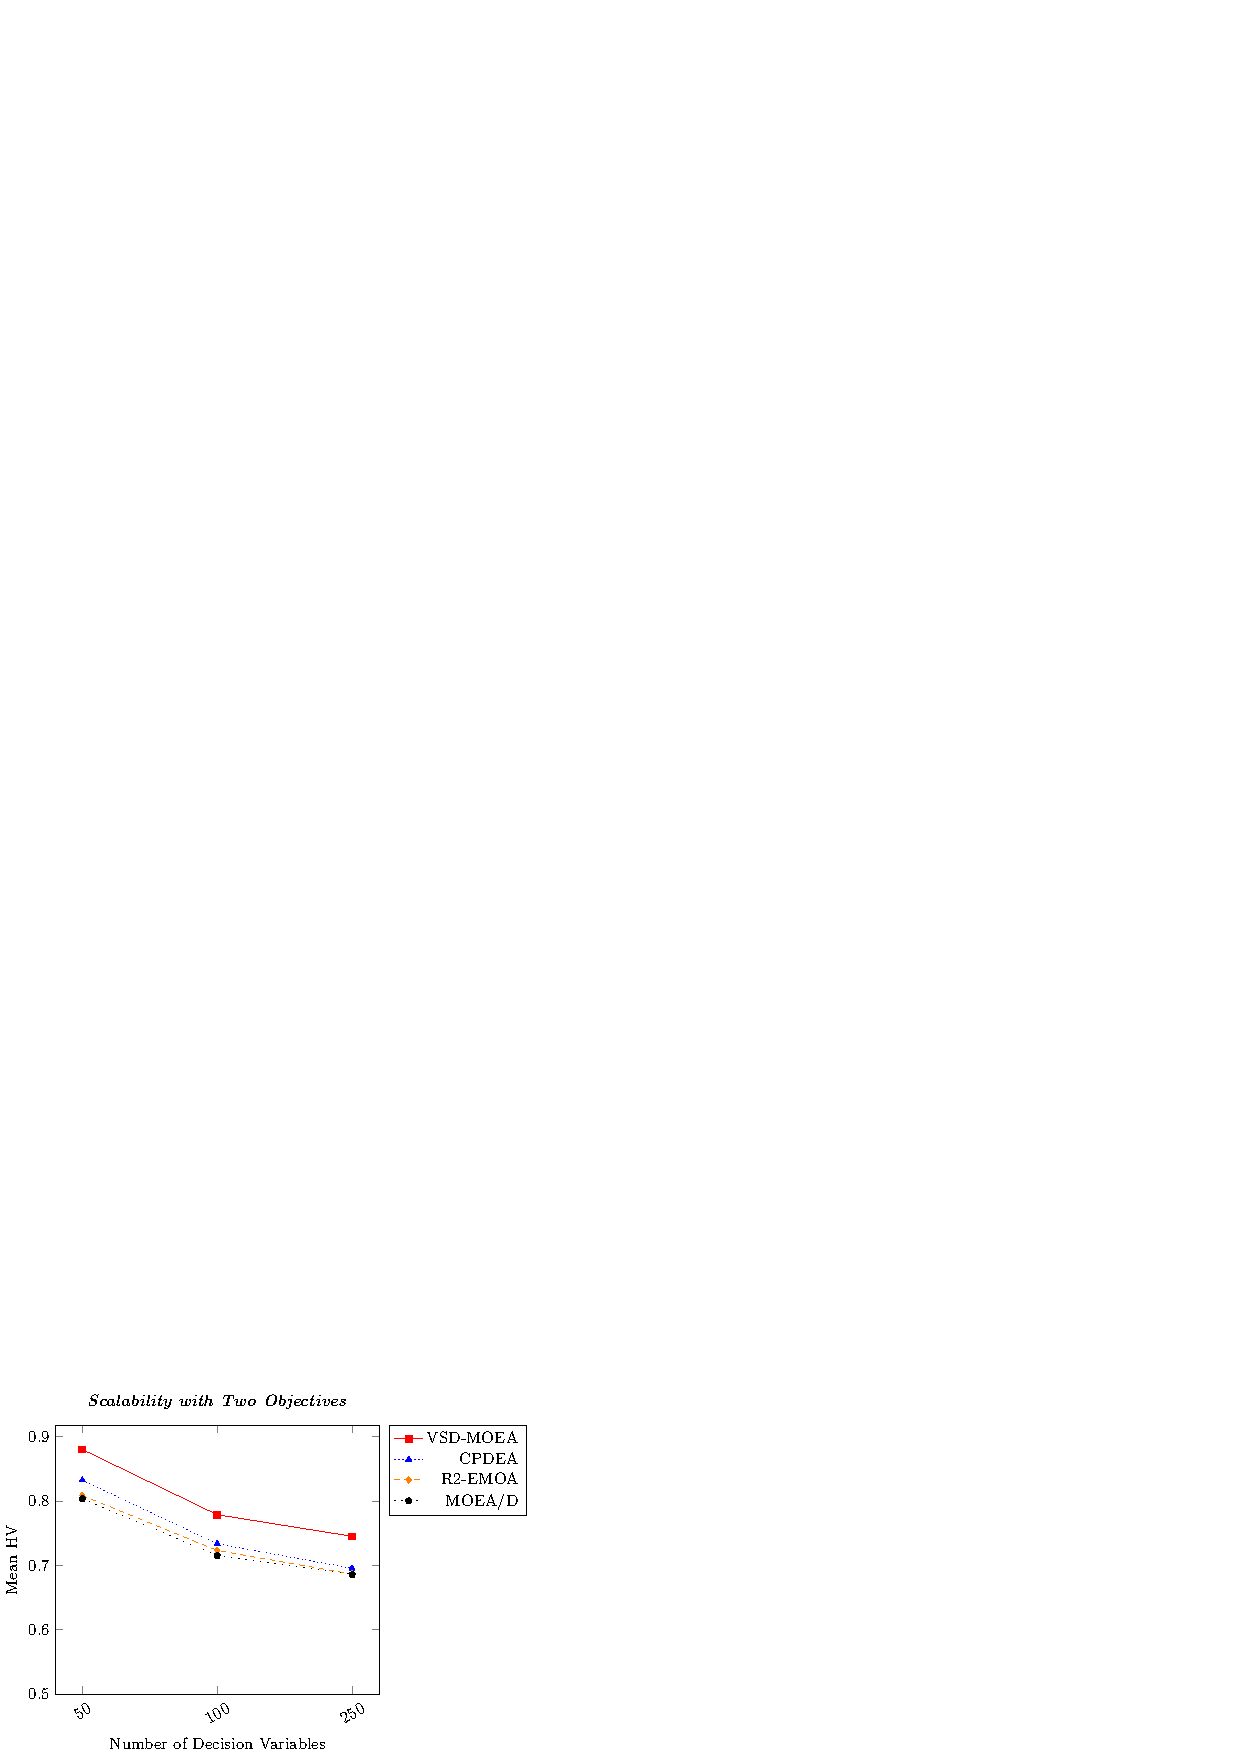
\includegraphics[]{Images/Graphic-Scalability-2obj_tikz-figure0.pdf}
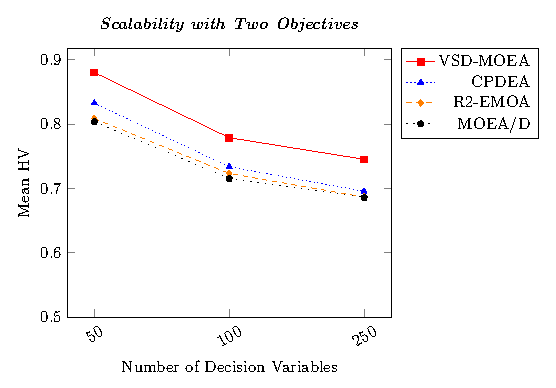
\includegraphics[]{Images/Graphic-Scalability-2obj_tikz-figure0.eps}
%\begin{tikzpicture}[scale=0.8]
\begin{axis}[
ymin=0.5,
%ymax=1.1,
%x label style={at={(current axis.left of origin)},anchor=north, below=10mm},
title={\textit{\textbf{Scalability with Two Objectives}}},
    xlabel=Number of Decision Variables,
  ylabel=Mean HV,
  xticklabel style = {rotate=30},
  legend style=
    {cells={anchor=east},legend pos=outer north east,},
  % enlargelimits = false,
  xticklabels from table={\ScalabilityTwoObj}{mean},xtick=data]
  
\addplot[red,solid,mark=square*] 
table [y=VSD_MOEA,x=X]{\ScalabilityTwoObj};
\addlegendentry{VSD-MOEA}
\addplot[blue,dotted,mark=triangle*] table[y= NSGA_II,x=X]{\ScalabilityTwoObj};
\addlegendentry{NSGA-II}]
		
\addplot[orange,dashed,mark=diamond*] table [y= R2_MOEA,x=X]{\ScalabilityTwoObj};
\addlegendentry{R2-MOEA}]
    
\addplot[black,loosely dotted,mark=pentagon*] table [y= MOEA_D,x=X]{\ScalabilityTwoObj};
\addlegendentry{MOEA/D}]
\end{axis}
\end{tikzpicture}
%\begin{tikzpicture}[scale=0.8]
%\begin{axis}[
%%ymin=0.5    ,
%%ymax=1.1,
%%x label style={at={(current axis.left of origin)},anchor=north, below=10mm},
%title={\textit{\textbf{Scalability UF5}}},
%    xlabel=Number of Decision Variables,
%  ylabel=Mean HV,
%  xticklabel style = {rotate=30},
%  legend style=
%    {cells={anchor=east},legend pos=outer north east,},
%  % enlargelimits = false,
%  xticklabels from table={\ScalabilityUFFiveTwoObj}{mean},xtick=data]
%  
%\addplot[red,solid,mark=square*] 
%table [y=VSD_MOEA,x=X]{\ScalabilityUFFiveTwoObj};
%\addlegendentry{VSD-MOEA}
%\addplot[blue,dotted,mark=triangle*] table [y= NSGA_II,x=X]{\ScalabilityUFFiveTwoObj};
%\addlegendentry{NSGA-II}]
%		
%\addplot[orange,dashed,mark=diamond*] table [y= R2_MOEA,x=X]{\ScalabilityUFFiveTwoObj};
%\addlegendentry{R2-MOEA}]
%    
%\addplot[black,loosely dotted,mark=pentagon*] table [y= MOEA_D,x=X]{\ScalabilityUFFiveTwoObj};
%\addlegendentry{MOEA/D}]
%\end{axis}
%\end{tikzpicture}
%\caption{Mean of the \HV{} (35 runs) considering two objectives.}

\caption{Mean of the \HV{} (35 runs) considering two objectives.}\label{fig:variable-decision-scalability-2obj}
\end{figure}

\begin{figure}[t]
\centering
%\includegraphics[]{Images/Graphic-Scalability-3obj_tikz-figure0.pdf}
\includegraphics[]{Images/Graphic-Scalability-3obj_tikz-figure0.eps}
%\begin{tikzpicture}[scale=0.8]
\begin{axis}[
ymin=0.0,
title={\textit{\textbf{Scalability with Three Objectives}}},
    xlabel=Number of Decision Variables,
  ylabel=Mean HV,
%  xlabel style={yshift=-0.2cm},
  xticklabel style = {rotate=30},
  legend style=
    {cells={anchor=east},legend pos=outer north east,},
  xticklabels from table={\ScalabilityThreeObj}{mean},xtick=data]
  
\addplot[red,solid,mark=square*] 
table [y=VSD_MOEA,x=X]{\ScalabilityThreeObj};
\addlegendentry{VSD-MOEA}
\addplot[blue,dotted,mark=triangle*] table [y= NSGA_II,x=X]{\ScalabilityThreeObj};
\addlegendentry{NSGA-II}]
		
\addplot[orange,dashed,mark=diamond*] table [y= R2_MOEA,x=X]{\ScalabilityThreeObj};
\addlegendentry{R2-MOEA}]
    
\addplot[black,loosely dotted,mark=pentagon*] table [y= MOEA_D,x=X]{\ScalabilityThreeObj};
\addlegendentry{MOEA/D}]
\end{axis}
\end{tikzpicture}
%\begin{tikzpicture}[scale=0.8]
%\begin{axis}[
%ymin=0.0,
%title={\textit{\textbf{Scalability UF10}}},
%    xlabel=Number of Decision Variables,
%  ylabel=Mean HV,
%  xticklabel style = {rotate=30},
%  legend style=
%    {cells={anchor=east},legend pos=outer north east,},
%  xticklabels from table={\ScalabilityUFTenThreeObj}{mean},xtick=data]
%  
%\addplot[red,solid,mark=square*] 
%table [y=VSD_MOEA,x=X]{\ScalabilityUFTenThreeObj};
%\addlegendentry{VSD-MOEA}
%\addplot[blue,dotted,mark=triangle*] table [y= NSGA_II,x=X]{\ScalabilityUFTenThreeObj};
%\addlegendentry{NSGA-II}]
%		
%\addplot[orange,dashed,mark=diamond*] table [y= R2_MOEA,x=X]{\ScalabilityUFTenThreeObj};
%\addlegendentry{R2-MOEA}]
%    
%\addplot[black,loosely dotted,mark=pentagon*] table [y= MOEA_D,x=X]{\ScalabilityUFTenThreeObj};
%\addlegendentry{MOEA/D}]
%\end{axis}
%\end{tikzpicture}
%\caption{Mean of the \HV{} (35 runs) considering three objectives.}

\caption{Mean of the \HV{} (35 runs) considering three objectives.} \label{fig:variable-decision-scalability-3obj}
\end{figure}

In order, to have a better understanding of the algorithms and following the guideline of middle-term executions, the diversity in the decision variable space with some WFG problems is calculated.
%
Particularly, these problems divide the decision variables in two kinds of parameters: the distance parameters and the position parameters.
%
A parameter $x_i$ is a distance parameter when for all parameter vectors $\vec{F}(\mathbf{x})$, modifying $x_i$ in $\vec{F}(\mathbf{x})$ results in a parameter vector that dominates $\vec{F}(\mathbf{x})$, is equivalent to $\vec{F}(\mathbf{x})$, or is dominated by $\vec{F}(\mathbf{x})$.
%
However, if $x_i$ is a position parameter, modifying $x_i$ in $\vec{F}(\mathbf{x})$ always results in a vector that is incomparable or equivalent to $\vec{F}(\mathbf{x})$~\cite{huband2005scalable}.
%

%
Particularly, the selected problems were used to show that either premature convergence or stagnation appears in the set of distance parameters.
%
Consequently, the operators involved lose its exploratory strength.
%
We select the WFG1-WFG7 problems because their distance parameters values associated to Pareto optimal solutions have exactly the same values.
%
This values is shown as follows:
\begin{equation}
   x_{i=k+1:n} = 2i \times 0.35
\end{equation}
%
%
In order to analyze the diversity, the average Euclidean distance among individuals (ADI) is calculated, i.e. the mean value of all pairwise distances among individuals in the population is reported.
%
In Figures \ref{fig:Diversity_2obj} and \ref{fig:Diversity_3obj} are shown the evolution of diversity with two and three objectives.
%
Concretely, each figure shows the diversity maintained in the position parameters and the distance parameters.
%
The diversity is calculated with $50$, $100$, and $250$ variables for each algorithm.
%
Mainly, the state-of-the-art algorithms converged to promising regions in the distance parameters after the $10\%$ of the total time-execution.
%
However, their diversity in position parameters increases as the time elapses, meaning that the remaining $90\%$ is devoted to promote diverse solutions in the objective space.
%
In spite this, it seems that the algorithms converge on the distance parameters to promising regions, even though those regions could not be the optimal.
%
In contrast, \VSDMOEA{} keeps diverse solutions in both kind of parameters until the $90\%$ of the time elapsed, this strategy allows to explore more adequately the promising regions and might avoid stagnation in several stages.
%
\begin{figure}[t]
\centering
%\begin{tikzpicture}[scale=0.8]
\begin{axis}[
title={\textit{\textbf{Diversity of the Position Variables with Two Objectives}}},
  xlabel=Generation,
  ylabel=ADI,
  xticklabel style = {rotate=30},
%  xlabel style={yshift=-0.2cm},
  legend style=
    {cells={anchor=east},legend pos=outer north east,}, nodes={scale=0.8, transform shape}    ,
  xticklabels from table={\DiversityTwoWFG}{mean},xtick=data]
 

\addplot[red,dotted,mark=square*] table [y=VSD_MOEA_Position_50,x=X]{\DiversityTwoWFG};
	\addlegendentry{VSD-MOEA (50)}

\addplot[blue,dotted,mark=triangle*] table[y= NSGA_II_Position_50,x=X]{\DiversityTwoWFG};
	\addlegendentry{NSGA-II (50)}
		
\addplot[orange,dotted,mark=diamond*] table [y= R2_MOEA_Position_50,x=X]{\DiversityTwoWFG};
	\addlegendentry{R2-EMOA (50)}
    
\addplot[black,dotted,mark=pentagon*] table [y= MOEA_D_Position_50,x=X]{\DiversityTwoWFG};
	\addlegendentry{MOEA/D (50)}


\addplot[red,solid,mark=square*] table [y=VSD_MOEA_Position_100,x=X]{\DiversityTwoWFG};
	\addlegendentry{VSD-MOEA (100)}

\addplot[blue,solid,mark=triangle*] table[y= NSGA_II_Position_100,x=X]{\DiversityTwoWFG};
	\addlegendentry{NSGA-II (100)}
		
\addplot[orange,solid,mark=diamond*] table [y= R2_MOEA_Position_100,x=X]{\DiversityTwoWFG};
	\addlegendentry{R2-EMOA (100)}
    
\addplot[black,solid,mark=pentagon*] table [y= MOEA_D_Position_100,x=X]{\DiversityTwoWFG};
	\addlegendentry{MOEA/D (100)}


\addplot[red,loosely dashdotted,mark=square*] table [y=VSD_MOEA_Position_250,x=X]{\DiversityTwoWFG};
	\addlegendentry{VSD-MOEA (250)}

\addplot[blue,loosely dashdotted,mark=triangle*] table[y= NSGA_II_Position_250,x=X]{\DiversityTwoWFG};
	\addlegendentry{NSGA-II (250)}
		
\addplot[orange,loosely dashdotted,mark=diamond*] table [y= R2_MOEA_Position_250,x=X]{\DiversityTwoWFG};
	\addlegendentry{R2-EMOA (250)}
    
\addplot[black,loosely dashdotted,mark=pentagon*] table [y= MOEA_D_Position_250,x=X]{\DiversityTwoWFG};
	\addlegendentry{MOEA/D (250)}



\end{axis}
\end{tikzpicture}


\begin{tikzpicture}[scale=0.8]
\begin{axis}[
title={\textit{\textbf{Diversity of the Distance Variables with Two Objectives}}},
  xlabel=Generation,
  ylabel=ADI,
%  xlabel style={yshift=-0.2cm},
  xticklabel style = {rotate=30},
  legend style=
    {cells={anchor=east},legend pos=outer north east,}, nodes={scale=0.8, transform shape}    ,
  xticklabels from table={\DiversityTwoWFG}{mean},xtick=data]

\addplot[red,dotted,mark=square*] table [y=VSD_MOEA_Distance_50,x=X]{\DiversityTwoWFG};
	\addlegendentry{VSD-MOEA (50)}

\addplot[blue,dotted,mark=triangle*] table[y= NSGA_II_Distance_50,x=X]{\DiversityTwoWFG};
	\addlegendentry{NSGA-II (50)}
		
\addplot[orange,dotted,mark=diamond*] table [y= R2_MOEA_Distance_50,x=X]{\DiversityTwoWFG};
	\addlegendentry{R2-EMOA (50)}
    
\addplot[black,dotted,mark=pentagon*] table [y= MOEA_D_Distance_50,x=X]{\DiversityTwoWFG};
	\addlegendentry{MOEA/D (50)}


\addplot[red,solid,mark=square*] table [y=VSD_MOEA_Distance_100,x=X]{\DiversityTwoWFG};
	\addlegendentry{VSD-MOEA (100)}

\addplot[blue,solid,mark=triangle*] table[y= NSGA_II_Distance_100,x=X]{\DiversityTwoWFG};
	\addlegendentry{NSGA-II (100)}
		
\addplot[orange,solid,mark=diamond*] table [y= R2_MOEA_Distance_100,x=X]{\DiversityTwoWFG};
	\addlegendentry{R2-EMOA (100)}
    
\addplot[black,solid,mark=pentagon*] table [y= MOEA_D_Distance_100,x=X]{\DiversityTwoWFG};
	\addlegendentry{MOEA/D (100)}


\addplot[red,loosely dashdotted,mark=square*] table [y=VSD_MOEA_Distance_250,x=X]{\DiversityTwoWFG};
	\addlegendentry{VSD-MOEA (250)}

\addplot[blue,loosely dashdotted,mark=triangle*] table[y= NSGA_II_Distance_250,x=X]{\DiversityTwoWFG};
	\addlegendentry{NSGA-II (250)}
		
\addplot[orange,loosely dashdotted,mark=diamond*] table [y= R2_MOEA_Distance_250,x=X]{\DiversityTwoWFG};
	\addlegendentry{R2-EMOA (250)}
    
\addplot[black,loosely dashdotted,mark=pentagon*] table [y= MOEA_D_Distance_250,x=X]{\DiversityTwoWFG};
	\addlegendentry{MOEA/D (250)}





\end{axis}
\end{tikzpicture}

%%\begin{tikzpicture}[scale=0.8]
%%\begin{axis}[
%%title={\textit{\textbf{Diversity of the Variables}}},
%%  xlabel=Generation,
%%  ylabel=ADI,
%%  xticklabel style = {rotate=30},
%%  legend style=
%%    {cells={anchor=east},legend pos=outer north east,},
%%  xticklabels from table={\DiversityTwoWFGOne}{mean},xtick=data]
%%
%%\addplot[red,dotted,mark=square*] table [y=VSD_MOEA,x=X]{\DiversityTwoWFGOne};
%%\addlegendentry{VSD-MOEA}
%%
%%\addplot[blue,dotted,mark=triangle*] table[y= NSGA_II,x=X]{\DiversityTwoWFGOne};
%%\addlegendentry{NSGA-II}
%%		
%%\addplot[orange,dotted,mark=diamond*] table [y= R2_MOEA,x=X]{\DiversityTwoWFGOne};
%%\addlegendentry{R2-MOEA}
%%    
%%\addplot[black,dotted,mark=pentagon*] table [y= MOEA_D,x=X]{\DiversityTwoWFGOne};
%%\addlegendentry{MOEA/D}
%%
%%
%%\addplot[red,solid,mark=square*] table [y=VSD_MOEA,x=X]{\DiversityThreeWFGOne};
%%\addlegendentry{VSD-MOEA}
%%
%%\addplot[blue,solid,mark=triangle*] table[y= NSGA_II,x=X]{\DiversityThreeWFGOne};
%%\addlegendentry{NSGA-II}
%%		
%%\addplot[orange,solid,mark=diamond*] table [y= R2_MOEA,x=X]{\DiversityThreeWFGOne};
%%\addlegendentry{R2-MOEA}
%%    
%%\addplot[black,solid,mark=pentagon*] table [y= MOEA_D,x=X]{\DiversityThreeWFGOne};
%%\addlegendentry{MOEA/D}
%%
%%	
%%\end{axis}
%%\end{tikzpicture}
%\caption{Evolution of Average Distance Individuals of the Problems WFG1-WFG7.}


%\includegraphics[]{Images/Graphic-Diversity_2obj_tikz-figure0.pdf} \\
\includegraphics[]{Images/Graphic-Diversity_2obj_tikz-figure0.eps} \\[0.2cm]
%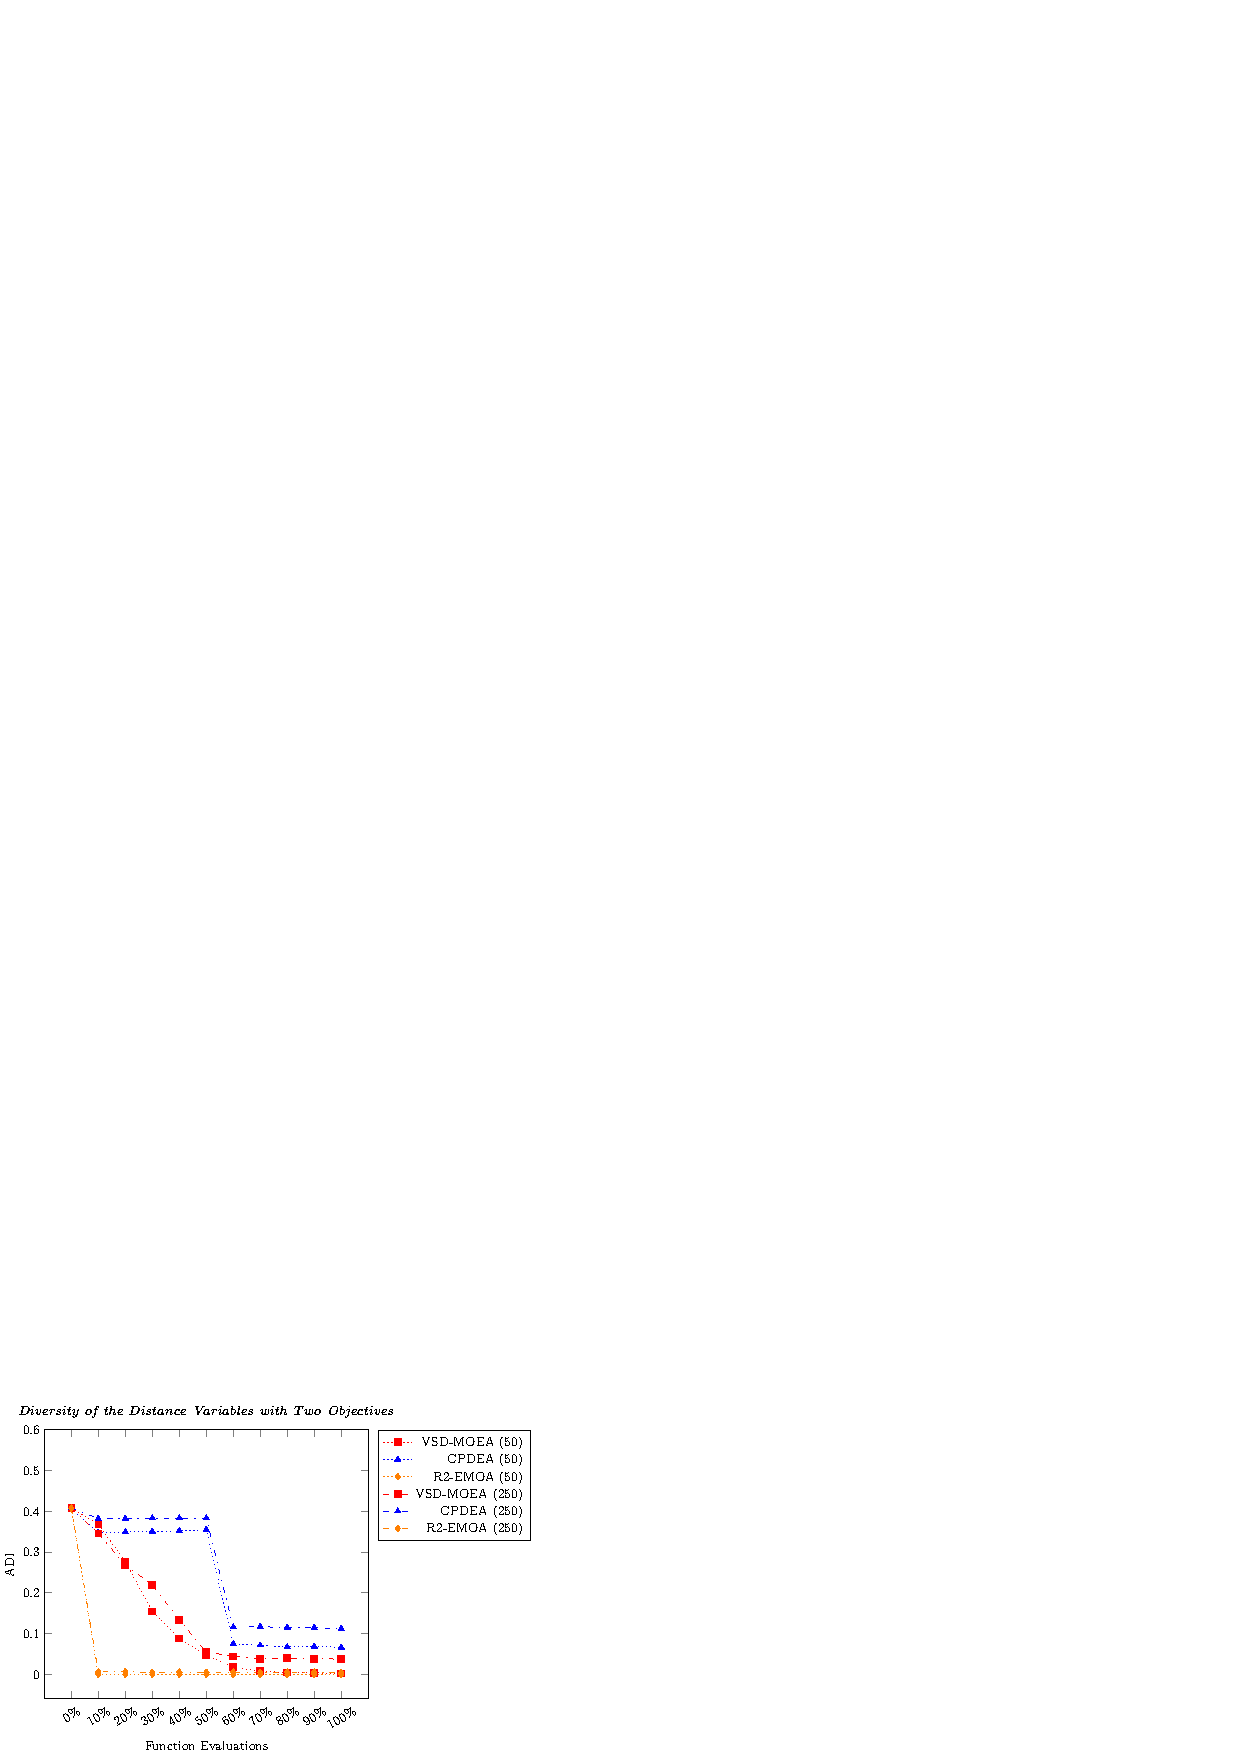
\includegraphics[]{Images/Graphic-Diversity_2obj_tikz-figure1.pdf}
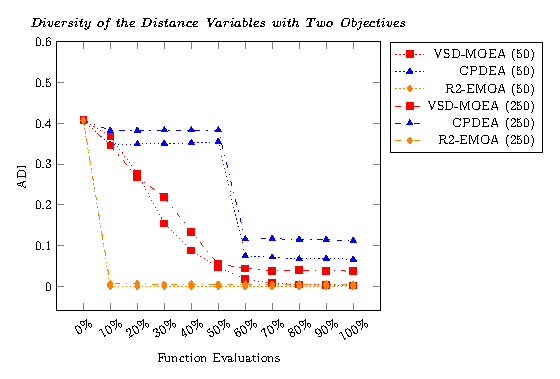
\includegraphics[]{Images/Graphic-Diversity_2obj_tikz-figure1.eps}
\caption{Evolution of average distance individuals of the problems WFG1-WFG7 with two objectives.}\label{fig:Diversity_2obj}
\end{figure}



In relation with the state-of-the-art algorithms, the diversity maintained in problems of three objectives was larger than with problems of two objectives, this might occurs since that the quantity of prominent solutions increases meaningfully between two and three objectives.
%
Therefore, there is present an implicit relation of diversity between the number of objectives and the decision variables space, in this situation three objectives keeps implicitly more diversity than two objectives.
%
However, this implicit diversity maintained is not enough to avoid stagnation in several problems.
%
Thus, the consideration of long-term executions in the state-of-the-art algorithms could not provide meaningfully improvements.
%
In contrast, \VSDMOEA{} could improve even more with long-term executions, since that it keeps diversity at several stages.
%
In general, as the number of variables is increased, the convergence in the distance parameters is even more slow, therefore to have quality solutions should be required a greater time-execution, specifically in the diversity-based approaches.
%

\begin{figure}[t]
\centering
%\input{Graphic-Diversity_3obj.tex}
%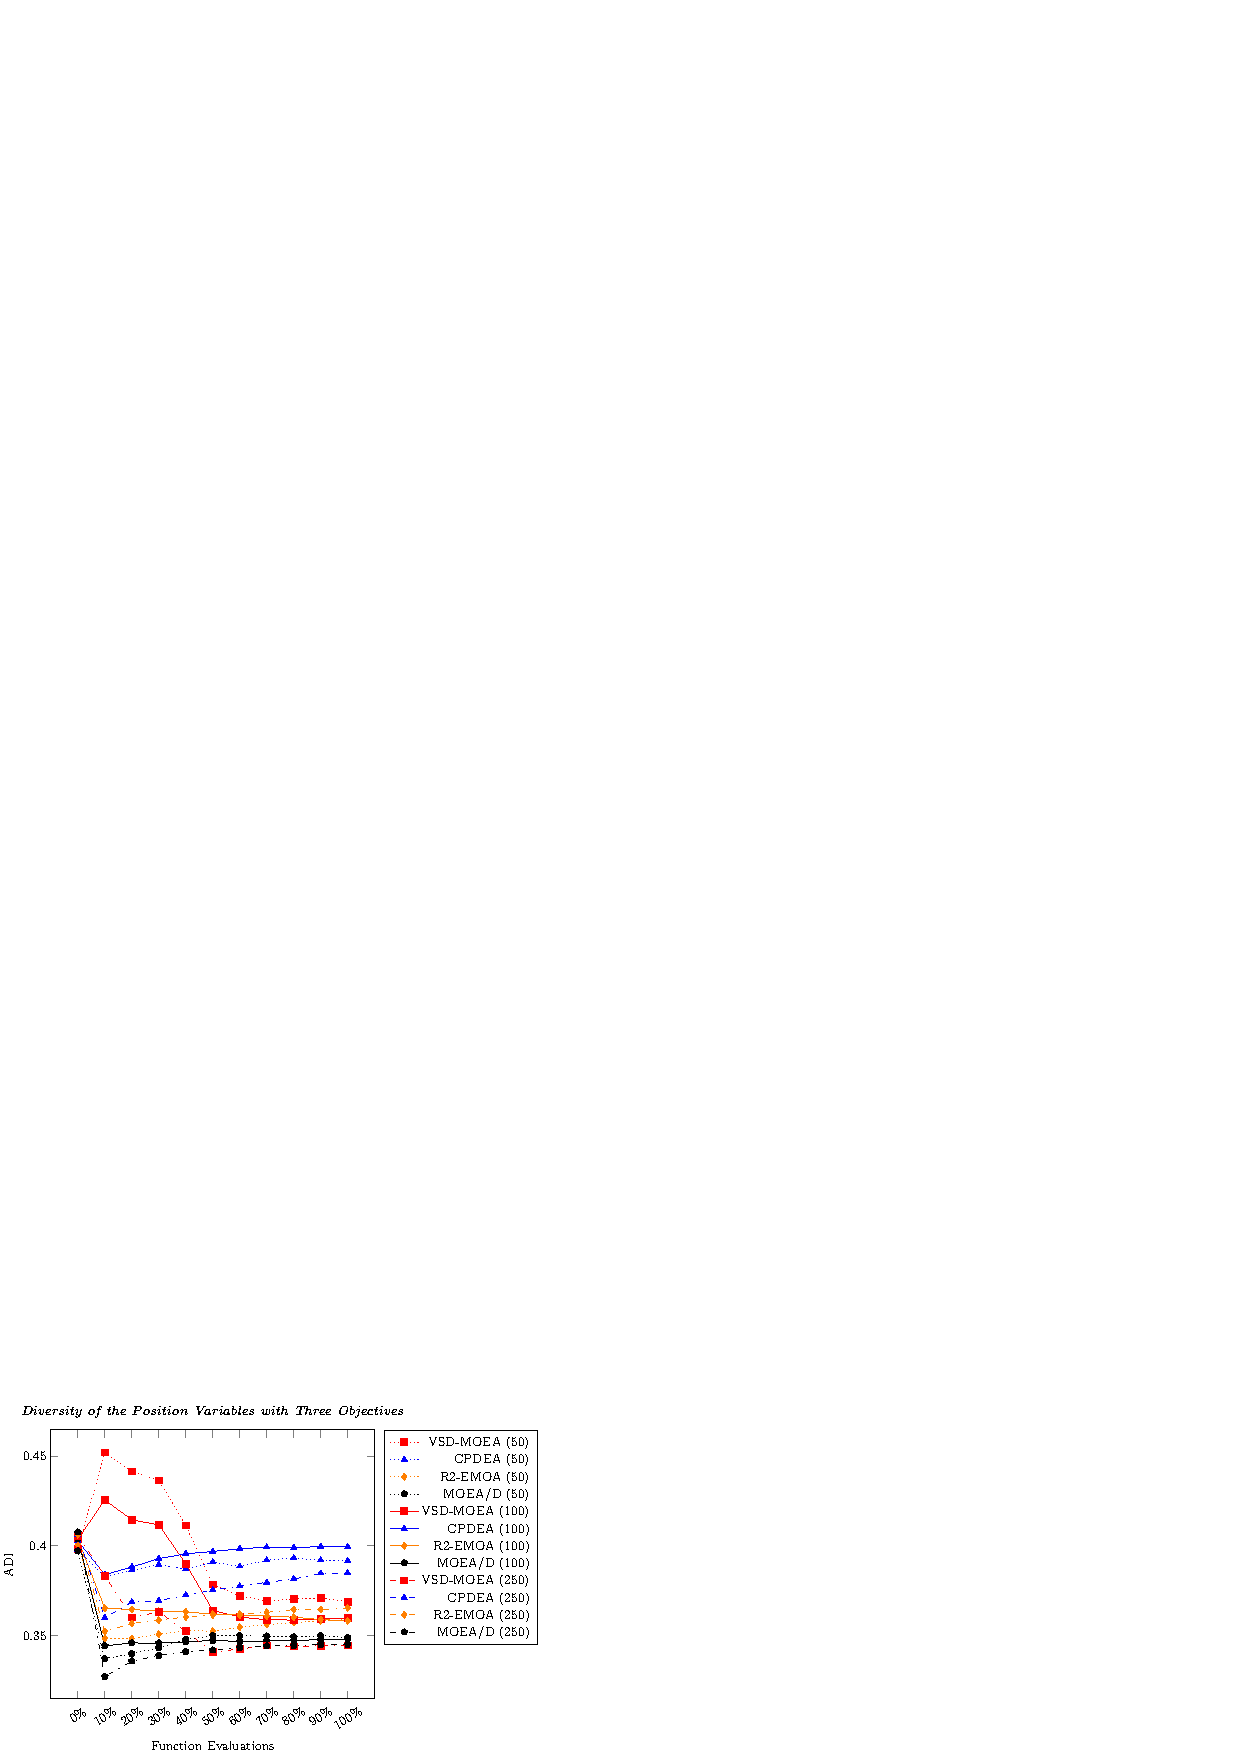
\includegraphics[]{Images/Graphic-Diversity_3obj_tikz-figure0.pdf} \\
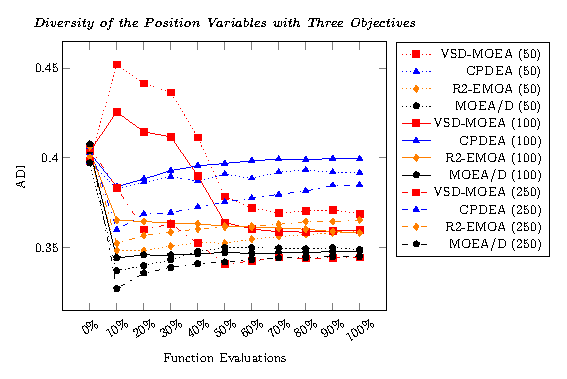
\includegraphics[]{Images/Graphic-Diversity_3obj_tikz-figure0.eps} \\[0.2cm]
%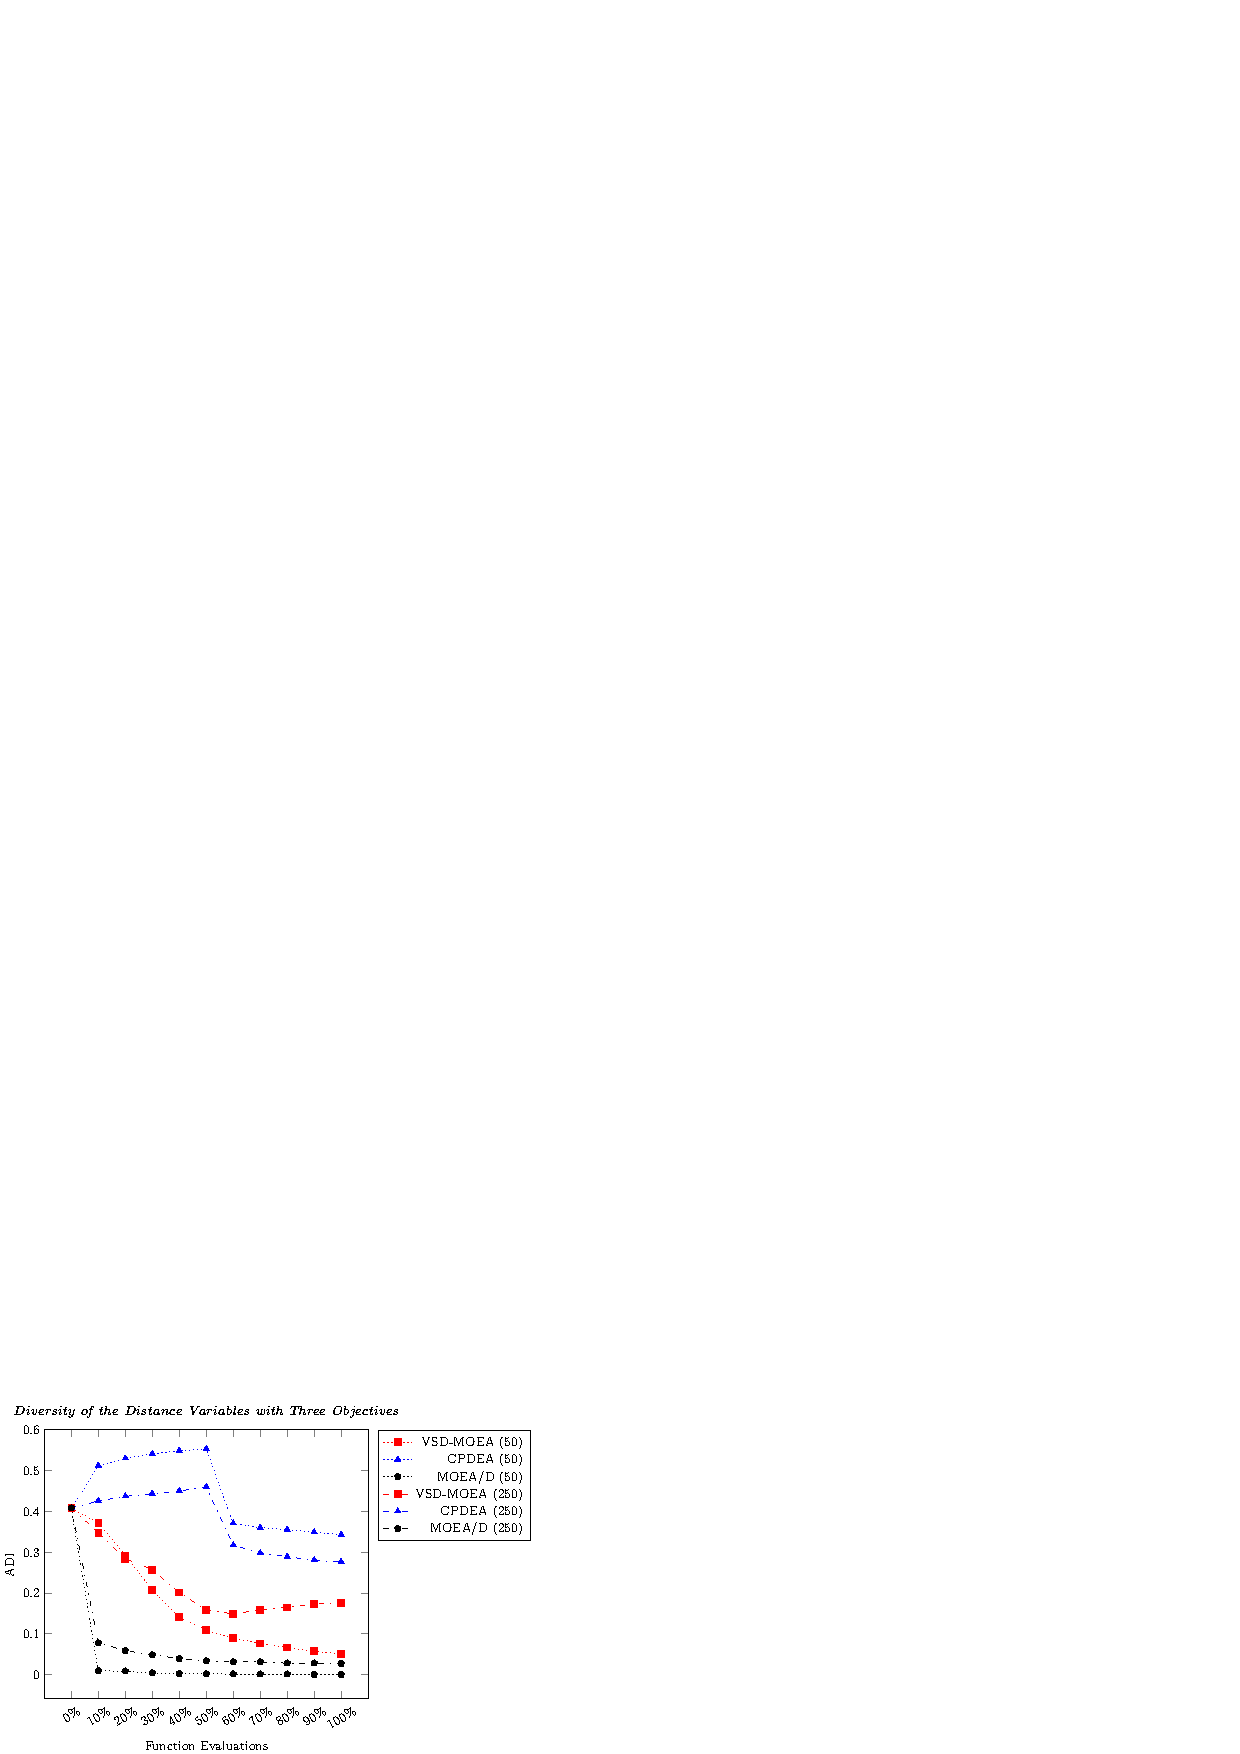
\includegraphics[]{Images/Graphic-Diversity_3obj_tikz-figure1.pdf}
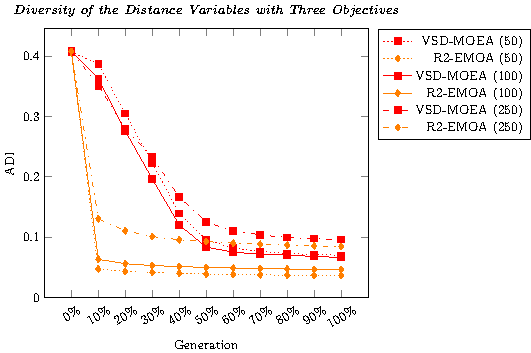
\includegraphics[]{Images/Graphic-Diversity_3obj_tikz-figure1.eps}
\caption{Evolution of average distance individuals of the problems WFG1-WFG7 with three objectives.}\label{fig:Diversity_3obj}
\end{figure}
%\begin{figure}[t]
%\centering
%\begin{tikzpicture}[scale=0.8]
\begin{axis}[
title={\textit{\textbf{Diversity of the Position Variables}}},
  xlabel=Generation,
  ylabel=ADI,
  xticklabel style = {rotate=30},
  legend style=
    {cells={anchor=east},legend pos=outer north east,},
  xticklabels from table={\DiversityTwoWFGSix}{mean},xtick=data]
 

\addplot[red,dotted,mark=square*] table [y=VSD_MOEA_Position,x=X]{\DiversityTwoWFGSix};
\addlegendentry{VSD-MOEA}

\addplot[blue,dotted,mark=triangle*] table[y= NSGA_II_Position,x=X]{\DiversityTwoWFGSix};
\addlegendentry{NSGA-II}
		
\addplot[orange,dotted,mark=diamond*] table [y= R2_MOEA_Position,x=X]{\DiversityTwoWFGSix};
\addlegendentry{R2-MOEA}
    
\addplot[black,dotted,mark=pentagon*] table [y= MOEA_D_Position,x=X]{\DiversityTwoWFGSix};
\addlegendentry{MOEA/D}


\addplot[red,solid,mark=square*] table [y=VSD_MOEA_Position,x=X]{\DiversityThreeWFGSix};
\addlegendentry{VSD-MOEA}

\addplot[blue,solid,mark=triangle*] table[y= NSGA_II_Position,x=X]{\DiversityThreeWFGSix};
\addlegendentry{NSGA-II}
		
\addplot[orange,solid,mark=diamond*] table [y= R2_MOEA_Position,x=X]{\DiversityThreeWFGSix};
\addlegendentry{R2-MOEA}
    
\addplot[black,solid,mark=pentagon*] table [y= MOEA_D_Position,x=X]{\DiversityThreeWFGSix};
\addlegendentry{MOEA/D}


\end{axis}
\end{tikzpicture}


\begin{tikzpicture}[scale=0.8]
\begin{axis}[
title={\textit{\textbf{Diversity of the Distance Variables}}},
  xlabel=Generation,
  ylabel=ADI,
  xticklabel style = {rotate=30},
  legend style=
    {cells={anchor=east},legend pos=outer north east,},
  xticklabels from table={\DiversityTwoWFGSix}{mean},xtick=data]

\addplot[red,dotted,mark=square*] table [y=VSD_MOEA_Distance,x=X]{\DiversityTwoWFGSix};
\addlegendentry{VSD-MOEA}

\addplot[blue,dotted,mark=triangle*] table[y= NSGA_II_Distance,x=X]{\DiversityTwoWFGSix};
\addlegendentry{NSGA-II}
		
\addplot[orange,dotted,mark=diamond*] table [y= R2_MOEA_Distance,x=X]{\DiversityTwoWFGSix};
\addlegendentry{R2-MOEA}
    
\addplot[black,dotted,mark=pentagon*] table [y= MOEA_D_Distance,x=X]{\DiversityTwoWFGSix};
\addlegendentry{MOEA/D}


\addplot[red,solid,mark=square*] table [y=VSD_MOEA_Distance,x=X]{\DiversityThreeWFGSix};
\addlegendentry{VSD-MOEA}

\addplot[blue,solid,mark=triangle*] table[y= NSGA_II_Distance,x=X]{\DiversityThreeWFGSix};
\addlegendentry{NSGA-II}
		
\addplot[orange,solid,mark=diamond*] table [y= R2_MOEA_Distance,x=X]{\DiversityThreeWFGSix};
\addlegendentry{R2-MOEA}
    
\addplot[black,solid,mark=pentagon*] table [y= MOEA_D_Distance,x=X]{\DiversityThreeWFGSix};
\addlegendentry{MOEA/D}

	
\end{axis}
\end{tikzpicture}

\begin{tikzpicture}[scale=0.8]
\begin{axis}[
title={\textit{\textbf{Diversity of the Variables}}},
  xlabel=Generation,
  ylabel=ADI,
  xticklabel style = {rotate=30},
  legend style=
    {cells={anchor=east},legend pos=outer north east,},
  xticklabels from table={\DiversityTwoWFGSix}{mean},xtick=data]

\addplot[red,dotted,mark=square*] table [y=VSD_MOEA,x=X]{\DiversityTwoWFGSix};
\addlegendentry{VSD-MOEA}

\addplot[blue,dotted,mark=triangle*] table[y= NSGA_II,x=X]{\DiversityTwoWFGSix};
\addlegendentry{NSGA-II}
		
\addplot[orange,dotted,mark=diamond*] table [y= R2_MOEA,x=X]{\DiversityTwoWFGSix};
\addlegendentry{R2-MOEA}
    
\addplot[black,dotted,mark=pentagon*] table [y= MOEA_D,x=X]{\DiversityTwoWFGSix};
\addlegendentry{MOEA/D}


\addplot[red,solid,mark=square*] table [y=VSD_MOEA,x=X]{\DiversityThreeWFGSix};
\addlegendentry{VSD-MOEA}

\addplot[blue,solid,mark=triangle*] table[y= NSGA_II,x=X]{\DiversityThreeWFGSix};
\addlegendentry{NSGA-II}
		
\addplot[orange,solid,mark=diamond*] table [y= R2_MOEA,x=X]{\DiversityThreeWFGSix};
\addlegendentry{R2-MOEA}
    
\addplot[black,solid,mark=pentagon*] table [y= MOEA_D,x=X]{\DiversityThreeWFGSix};
\addlegendentry{MOEA/D}

	
\end{axis}
\end{tikzpicture}

\caption{Evolution of the diversity for the problem WFG6}


%\label{fig:Diversity_WFG6}
%\end{figure}

\subsection{Performance of \MOEAS{} Through the Execution}


This section is devoted to test the performance of the algorithms with several stopping criteria, i.e. maximum number of generations.
%
As it is previously discussed, state-of-the-art algorithms might suffer of premature convergence or stagnation.
%
Therefore, the solutions could converge to promising --but not optimal-- regions at the first stages of the execution, wasting a meaningful quantity of generations.
%
To deal with this issue, \VSDMOEA{} maintains diversity at different stages as long as the stopping criterion is reached.
%
Accordingly, to have a better understanding of the performance obtained in each algorithm several stopping criteria have been probed.
%
In those runs the mean of normalized \HV{} of all the problems for two and three objectives are calculated.
%
Mainly, three ranges of stopping criterion were explored.
%
Each range was split in ten intervals, such ranges considered were $[250, 2500]$, $[2500, 25000]$ and $[25000, 250000]$ that are named as short-term, middle-term and long-term executions respectively.
%
In Figures \ref{fig:Performance_time_2obj} and \ref{fig:Performance_time_3obj} are showed the mean \HV{} values attained with each \MOEA{} with two and three objectives respectively.
%
Each figure is conformed by three graphics which correspond to short-term, middle-term and long-term.
%
Those figures demonstrate that \VSDMOEA{} attained competitive results considering short-term executions.
%
Even more, as the maximum number of generations is increased its performance is improved.
%
In fact after $2,500$ generations \VSDMOEA{} has a notorious improvement respect to the state-of-the-art-\MOEAS{} in both two and three objectives (second row of Figures \ref{fig:Performance_time_2obj} and \ref{fig:Performance_time_3obj}).
%
In problems of two objectives state-of-the-art algorithms attained quite similar \HV{} values in long-term executions ($250,000$ generations).
%
The weight-vector based algorithms had a similar behavior modificating the stopping criterion.
%
Particularly, \RMOEA{} improved state-of-the-art algorithms with problems of three objectives (Figure \ref{fig:Performance_time_3obj}).
%
Moreover, this algorithm showed a lightly constant improvement increasing the number of generations.
%
However, \VSDMOEA{} attained the best results in long-term executions and could improve even more increasing the time-execution.
%


\begin{figure}[t]
\centering
%\begin{tikzpicture}[scale=0.8]
\begin{axis}[
title={\textit{\textbf{Performance of the algorithms with Two Objectivessss}}},
  xlabel= Maximum Number of Generations,
  ylabel=Mean HV,
%  ymin=0.3,
  ymax=1.0,
  xticklabel style = {rotate=90, anchor=east, font=\footnotesize,},
%  label style = {font=\small, },
  xlabel style={yshift=-0.5cm},
%  xmode=log,
%  log basis x={2},
  legend style=
    {cells={anchor=east},legend pos=outer north east,},
  xticklabels from table={\Performancetimetwo}{mean},xtick=data]
 

\addplot[red,dotted,mark=square*] table [y=VSD_MOEA,x=X]{\Performancetimetwo};
\addlegendentry{VSD-MOEA}

\addplot[blue,dotted,mark=triangle*] table[y= NSGA_II,x=X]{\Performancetimetwo};
\addlegendentry{NSGA-II}
		
\addplot[orange,dotted,mark=diamond*] table [y= R2_MOEA,x=X]{\Performancetimetwo};
\addlegendentry{R2-MOEA}
    
\addplot[black,dotted,mark=pentagon*] table [y= MOEA_D,x=X]{\Performancetimetwo};
\addlegendentry{MOEA/D}
\draw [red, dashed] (axis cs:10, 0) -- (axis cs:10, 1);
\draw [red, dashed] (axis cs:19, 0) -- (axis cs:19, 1);
\end{axis}
\end{tikzpicture}


\begin{tikzpicture}[scale=0.8]
\begin{axis}[
title={\textit{\textbf{Performance of the algorithms with Three Objectives}}},
  xlabel= Maximum Number of Generations,
  ylabel=Mean HV,
%  ymin=0.5,
 % ymax=1.0,
  xticklabel style = {rotate=90, anchor=east, font=\footnotesize,},
  xlabel style={yshift=-0.5cm},
  legend style=
    {cells={anchor=east},legend pos=outer north east,},
  xticklabels from table={\Performancetimethree}{mean},xtick=data]

\addplot[red,dashed,mark=square*] table [y=VSD_MOEA,x=X]{\Performancetimethree};
\addlegendentry{VSD-MOEA}

\addplot[blue,dashed,mark=triangle*] table[y= NSGA_II,x=X]{\Performancetimethree};
\addlegendentry{NSGA-II}
		
\addplot[orange,dashed,mark=diamond*] table [y= R2_MOEA,x=X]{\Performancetimethree};
\addlegendentry{R2-MOEA}
    
\addplot[black,dashed,mark=pentagon*] table [y= MOEA_D,x=X]{\Performancetimethree};
\addlegendentry{MOEA/D};
\draw [red, dashed] (axis cs:10, 0) -- (axis cs:10, 1);
\draw [red, dashed] (axis cs:19, 0) -- (axis cs:19, 1);
\end{axis}
\end{tikzpicture}



%\caption{Performance of the \MOEAS{} considerin several maximum number of generations.}

%\includegraphics[angle=90,origin=c]{Images/Graphic-Performance-Time_tikz-figure0.pdf} \\
%\includegraphics[angle=90,origin=c]{Images/Graphic-Performance-Time_tikz-figure0.eps} \\
\begin{tabular}{l}
 \includegraphics[scale=0.6]{Images/Time_tikz-figure0.eps}\\[0cm]%[-0.14cm] 
 \includegraphics[scale=0.6]{Images/Time_tikz-figure1.eps}\\[0cm]%[-0.18cm]
 \includegraphics[scale=0.6]{Images/Time_tikz-figure2.eps}
\end{tabular}
%\includegraphics[angle=90,origin=c]{Images/Graphic-Performance-Time_tikz-figure1.pdf} \\
%\includegraphics[angle=90,origin=c]{Images/Graphic-Performance-Time_tikz-figure1.eps}
\caption{Performance of the \MOEAS{} considering three ranges of stopping criterion. The configurations take place with short-term (first row), middle-term (second row) and long-term (third row) executions.}\label{fig:Performance_time_2obj}
\end{figure}

\begin{figure}[t]
\centering
%\begin{tikzpicture}[scale=0.8]
\begin{axis}[
title={\textit{\textbf{Performance of the algorithms with Two Objectivessss}}},
  xlabel= Maximum Number of Generations,
  ylabel=Mean HV,
%  ymin=0.3,
  ymax=1.0,
  xticklabel style = {rotate=90, anchor=east, font=\footnotesize,},
%  label style = {font=\small, },
  xlabel style={yshift=-0.5cm},
%  xmode=log,
%  log basis x={2},
  legend style=
    {cells={anchor=east},legend pos=outer north east,},
  xticklabels from table={\Performancetimetwo}{mean},xtick=data]
 

\addplot[red,dotted,mark=square*] table [y=VSD_MOEA,x=X]{\Performancetimetwo};
\addlegendentry{VSD-MOEA}

\addplot[blue,dotted,mark=triangle*] table[y= NSGA_II,x=X]{\Performancetimetwo};
\addlegendentry{NSGA-II}
		
\addplot[orange,dotted,mark=diamond*] table [y= R2_MOEA,x=X]{\Performancetimetwo};
\addlegendentry{R2-MOEA}
    
\addplot[black,dotted,mark=pentagon*] table [y= MOEA_D,x=X]{\Performancetimetwo};
\addlegendentry{MOEA/D}
\draw [red, dashed] (axis cs:10, 0) -- (axis cs:10, 1);
\draw [red, dashed] (axis cs:19, 0) -- (axis cs:19, 1);
\end{axis}
\end{tikzpicture}


\begin{tikzpicture}[scale=0.8]
\begin{axis}[
title={\textit{\textbf{Performance of the algorithms with Three Objectives}}},
  xlabel= Maximum Number of Generations,
  ylabel=Mean HV,
%  ymin=0.5,
 % ymax=1.0,
  xticklabel style = {rotate=90, anchor=east, font=\footnotesize,},
  xlabel style={yshift=-0.5cm},
  legend style=
    {cells={anchor=east},legend pos=outer north east,},
  xticklabels from table={\Performancetimethree}{mean},xtick=data]

\addplot[red,dashed,mark=square*] table [y=VSD_MOEA,x=X]{\Performancetimethree};
\addlegendentry{VSD-MOEA}

\addplot[blue,dashed,mark=triangle*] table[y= NSGA_II,x=X]{\Performancetimethree};
\addlegendentry{NSGA-II}
		
\addplot[orange,dashed,mark=diamond*] table [y= R2_MOEA,x=X]{\Performancetimethree};
\addlegendentry{R2-MOEA}
    
\addplot[black,dashed,mark=pentagon*] table [y= MOEA_D,x=X]{\Performancetimethree};
\addlegendentry{MOEA/D};
\draw [red, dashed] (axis cs:10, 0) -- (axis cs:10, 1);
\draw [red, dashed] (axis cs:19, 0) -- (axis cs:19, 1);
\end{axis}
\end{tikzpicture}



%\caption{Performance of the \MOEAS{} considerin several maximum number of generations.}

%\includegraphics[angle=90,origin=c]{Images/Graphic-Performance-Time_tikz-figure0.pdf} \\
%\includegraphics[angle=90,origin=c]{Images/Graphic-Performance-Time_tikz-figure0.eps} \\
\begin{tabular}{l}
 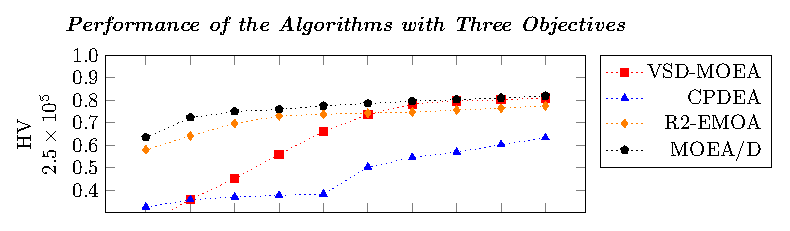
\includegraphics[scale=0.6]{Images/Time_tikz-figure3.eps}\\[0cm]%[-0.14cm] 
 \includegraphics[scale=0.6]{Images/Time_tikz-figure4.eps}\\[0cm]%[-0.18cm]
 \includegraphics[scale=0.6]{Images/Time_tikz-figure5.eps}
\end{tabular}
\caption{Performance of the \MOEAS{} considering three ranges of stopping criterion. The configurations take place with short-term (first row), middle-term (second row) and long-term (third row) executions.}\label{fig:Performance_time_3obj}
\end{figure}


\subsection{Analysis of the Initial Threshold Value}

Avoidance of premature convergence and stagnation in long-term executions is a difficult task mainly in multi-objective problems since that --depending of the problem-- the objective space implicitly involves a relation of diversity in the decision variable space.
%
For this reason, a potential strategy to mitigate those drawbacks is to lead the algorithm through different diversity stages and taking into account the stopping criterion to stimulate an appropriate balance between exploration and exploitation.
%
Nevertheless, the latter strategy, which is Incorporated in \VSDMOEA{}, requires an initial parameter, which represents the initial diversity induced in the algorithm, better known as the initial threshold value ($D_I$).
%
Accordingly, this initial threshold value is decreasing as the time elapses.
%
In order, to have a better insight about the effect raised of inducing several initial diversity stages, \VSDMOEA{} is tested with several initial threshold values and in long-term executions ($250,000$ generations).
%
Particularly, this parameter is computed as a fraction of the main normalized diagonal, which belongs to the unitary hyper-cube, the portions considered are $D_I = \{0.0, 0.1, 0.2, 0.3, 0.4, 0.5, 0.6, 0.7, 0.8, 0.9\}$.
%
In Figure \ref{fig:Initial-distance-factor} is shown the general normalized mean of the \HV{} for each configuration with two an three objectives.
%
Specifically, setting $D_I=0.0$ implies that the diversity is not promoted resulting in a similar behavior as the dominance-based algorithm.
%
In spite of this setting, \VSDMOEA{} attained better \HV{} values with all the settings than the state-of-the-art algorithms, in fact the lowest values were attained without inducing diversity, such values were $0.912$ and $0.893$ for two and three objectives respectively.
%
Especially, the maximum benefit achieved of inducing diversity is found with an initial threshold value of $DI=0.4$ with two and three objectives.
%
In addition, the behavior of setting several initial threshold value is quite similar with two and three objectives.
%
Therefore, inducing diversity and taking into account the elapses generations can be useful mainly for middle-term and long-term executions.

\begin{figure}[t]
\centering
%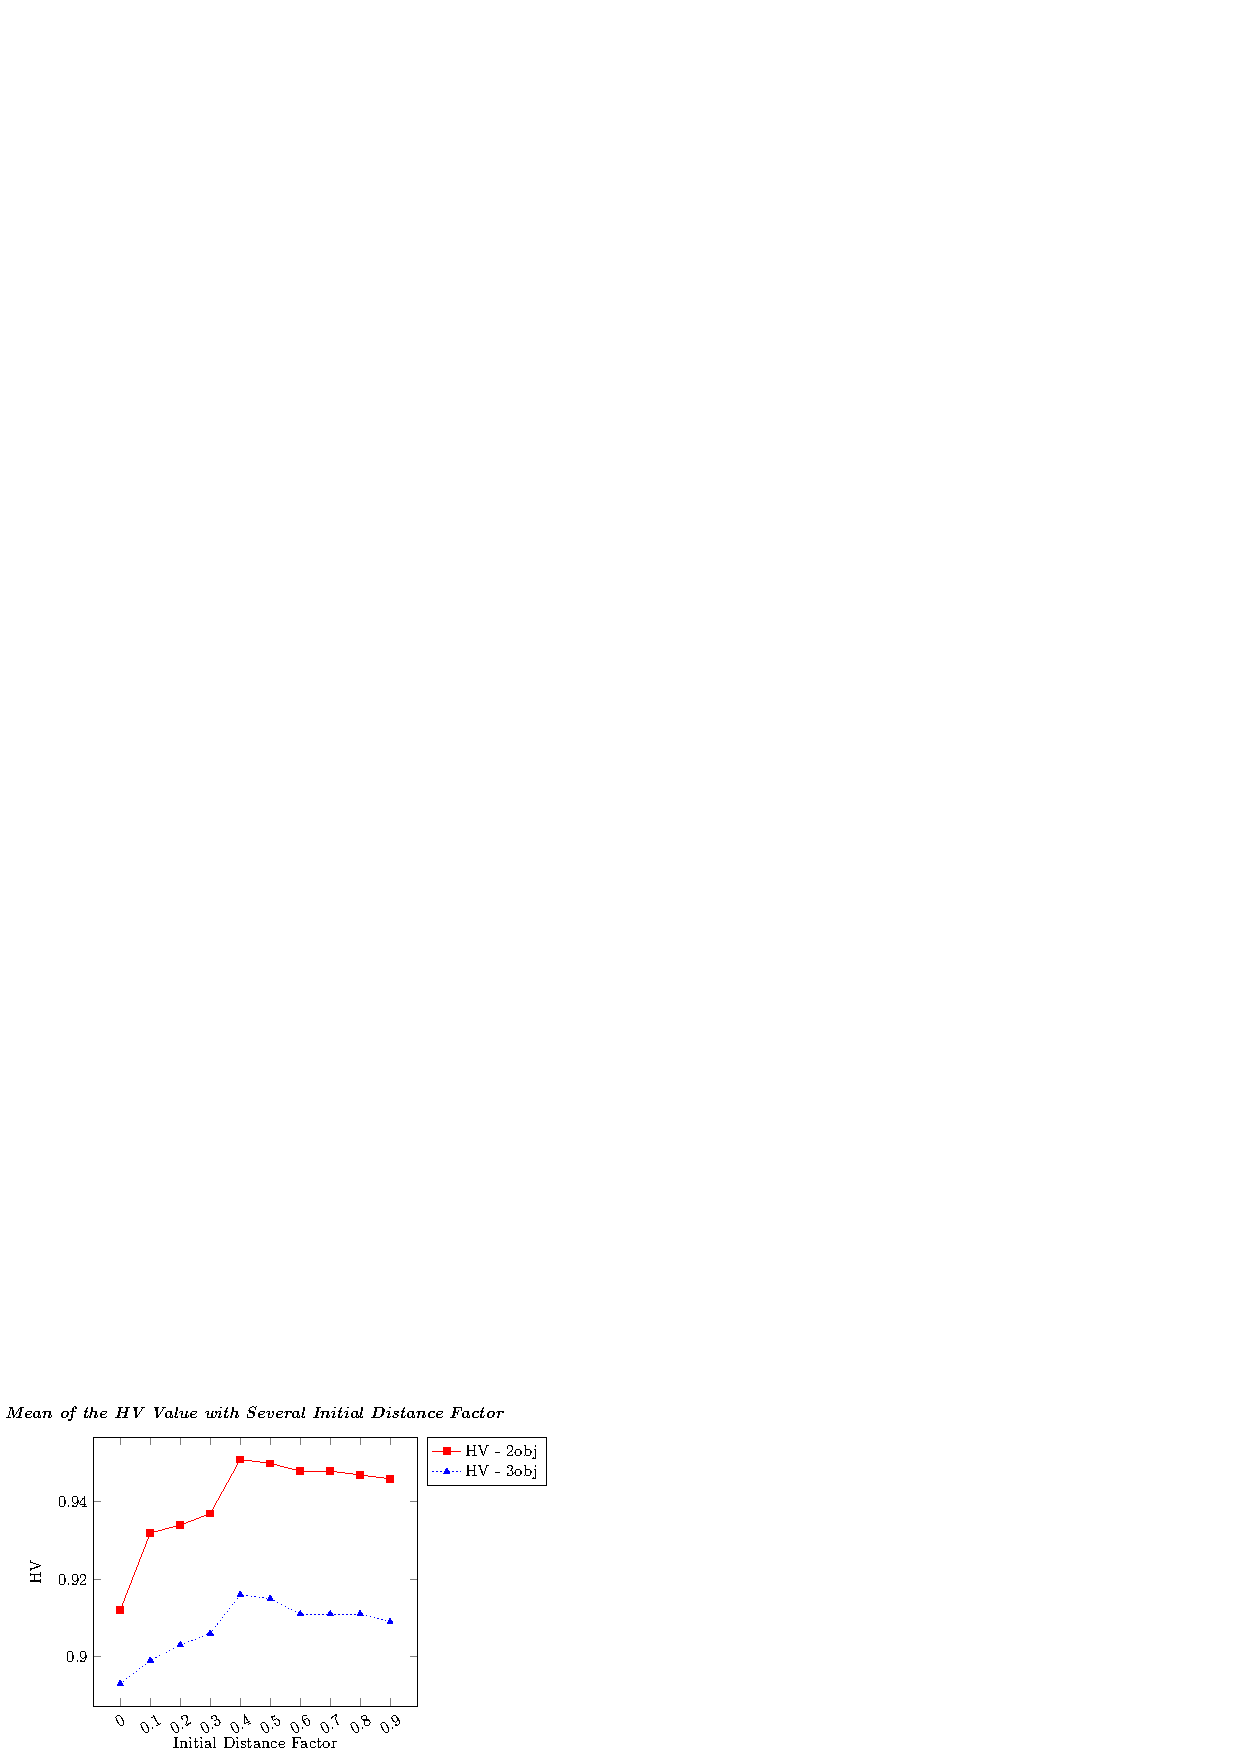
\includegraphics[]{Images/Graphic-Initial-Distance_tikz-figure0.pdf} \\
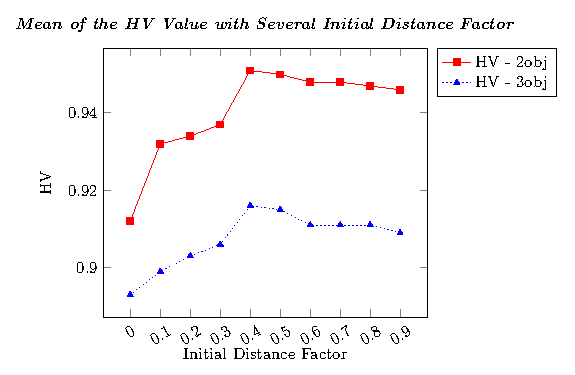
\includegraphics[]{Images/Graphic-Initial-Distance_tikz-figure0.eps} \\
%\begin{tikzpicture}[scale=0.8]
\begin{axis}[
title={\textit{\textbf{Mean of the HV Value with Several Initial Threshold Values}}},
    xlabel=Initial Threshold Value,
  ylabel=HV,
%  xlabel style={yshift=-0.2cm},
  xticklabel style = {rotate=30},
  legend style=
    {cells={anchor=east},legend pos=outer north east,},
  xticklabels from table={\DIHV}{mean},xtick=data]
  
\addplot[red,solid,mark=square*] 
table [y=HV2obj,x=X]{\DIHV};
\addlegendentry{HV - 2obj}
\addplot[blue,dotted,mark=triangle*] table[y= HV3obj,x=X]{\DIHV};
\addlegendentry{HV - 3obj}
		
\end{axis}
\end{tikzpicture}
%%\begin{tikzpicture}[scale=0.8]
%%\begin{axis}[
%%ymin=0.0    ,
%%ymax=0.1,
%%title={\textit{\textbf{Mean of the IGD+ Value with Several Initial Distance Factor}}},
%%    xlabel=Initial Distance Factor,
%%  ylabel=IGD+,
%%  xticklabel style = {rotate=30},
%%  legend style=
%%    {cells={anchor=east},legend pos=outer north east,},
%%  xticklabels from table={\DIIGDP}{mean},xtick=data]
%%\addplot[red,solid,mark=square*] 
%%table [y=IGD2obj,x=X]{\DIIGDP};
%%\addlegendentry{IGD+ 2obj}
%%\addplot[blue,dotted,mark=triangle*] table [y=IGD3obj,x=X]{\DIIGDP};
%%\addlegendentry{IGD+ 3obj}
%%\end{axis}
%%\end{tikzpicture}
%\caption{Mean of Inidicator Considering All Instances with Several Initial Distance Factors}

\caption{Mean of \HV{} values taking into account all instances with several initial threshold values.}\label{fig:Initial-distance-factor}
\end{figure}



% Please add the following required packages to your document preamble:
% \usepackage{graphicx}
\begin{table*}[t]
\caption{Summary of the hypervolume ratio results attained for problems with two objectives, the higher the normalized hypervolume value the better the algorithm.}
\label{tab:StatisticsHV_2obj}
%\resizebox{\textwidth}{!}{%
\begin{tabular}{cc|c|c|c|c|c|c|c}
\cline{2-9}
\textbf{}                           & \multicolumn{2}{c|}{\textbf{VSD-MOEA}}              & \multicolumn{2}{c|}{\textbf{CPDEA}} & \multicolumn{2}{c|}{\textbf{MOEA/D}} & \multicolumn{2}{c}{\textbf{R2-EMOA}} \\ \cline{2-9} 
\textbf{}                           & \multicolumn{1}{c|}{\textbf{Mean}}  & \textbf{Std} & \textbf{Mean}     & \textbf{Std}    & \textbf{Mean}      & \textbf{Std}    & \textbf{Mean}      & \textbf{Std}     \\ \hline
\multicolumn{1}{c|}{\textbf{WFG1}}  & \multicolumn{1}{c|}{\textbf{0.993}} & 0.002        & 0.963             & 0.013           & \textbf{0.993}     & 0.001           & 0.980              & 0.018            \\ \hline
\multicolumn{1}{c|}{\textbf{WFG2}}  & \multicolumn{1}{c|}{\textbf{0.996}} & 0.008        & 0.993             & 0.009           & 0.965              & 0.000           & 0.966              & 0.005            \\ \hline
\multicolumn{1}{c|}{\textbf{WFG3}}  & \multicolumn{1}{c|}{\textbf{0.992}} & 0.000        & 0.973             & 0.002           & \textbf{0.992}     & 0.000           & 0.991              & 0.000            \\ \hline
\multicolumn{1}{c|}{\textbf{WFG4}}  & \multicolumn{1}{c|}{0.990}          & 0.000        & 0.964             & 0.003           & 0.988              & 0.000           & \textbf{0.991}     & 0.000            \\ \hline
\multicolumn{1}{c|}{\textbf{WFG5}}  & \multicolumn{1}{c|}{0.880}          & 0.003        & 0.862             & 0.002           & 0.877              & 0.003           & \textbf{0.882}     & 0.002            \\ \hline
\multicolumn{1}{c|}{\textbf{WFG6}}  & \multicolumn{1}{c|}{0.884}          & 0.012        & 0.787             & 0.003           & \textbf{0.918}     & 0.020           & 0.914              & 0.015            \\ \hline
\multicolumn{1}{c|}{\textbf{WFG7}}  & \multicolumn{1}{c|}{0.990}          & 0.000        & 0.973             & 0.002           & 0.988              & 0.000           & \textbf{0.991}     & 0.000            \\ \hline
\multicolumn{1}{c|}{\textbf{WFG8}}  & \multicolumn{1}{c|}{\textbf{0.904}} & 0.053        & 0.875             & 0.026           & 0.808              & 0.007           & 0.803              & 0.005            \\ \hline
\multicolumn{1}{c|}{\textbf{WFG9}}  & \multicolumn{1}{c|}{\textbf{0.946}} & 0.027        & 0.791             & 0.002           & 0.912              & 0.070           & 0.894              & 0.079            \\ \hline
\multicolumn{1}{c|}{\textbf{DTLZ1}} & \multicolumn{1}{c|}{0.992}          & 0.000        & 0.991             & 0.000           & \textbf{0.993}     & 0.000           & 0.992              & 0.000            \\ \hline
\multicolumn{1}{c|}{\textbf{DTLZ2}} & \multicolumn{1}{c|}{0.990}          & 0.000        & 0.983             & 0.001           & 0.989              & 0.000           & \textbf{0.992}     & 0.000            \\ \hline
\multicolumn{1}{c|}{\textbf{DTLZ3}} & \multicolumn{1}{c|}{0.990}          & 0.000        & 0.988             & 0.000           & 0.989              & 0.000           & \textbf{0.992}     & 0.000            \\ \hline
\multicolumn{1}{c|}{\textbf{DTLZ4}} & \multicolumn{1}{c|}{\textbf{0.990}} & 0.000        & 0.979             & 0.003           & 0.989              & 0.000           & 0.678              & 0.362            \\ \hline
\multicolumn{1}{c|}{\textbf{DTLZ5}} & \multicolumn{1}{c|}{0.990}          & 0.000        & 0.983             & 0.001           & 0.989              & 0.000           & \textbf{0.992}     & 0.000            \\ \hline
\multicolumn{1}{c|}{\textbf{DTLZ6}} & \multicolumn{1}{c|}{\textbf{0.990}} & 0.000        & 0.807             & 0.088           & 0.989              & 0.000           & 0.685              & 0.088            \\ \hline
\multicolumn{1}{c|}{\textbf{DTLZ7}} & \multicolumn{1}{c|}{0.996}          & 0.000        & 0.995             & 0.000           & 0.996              & 0.000           & \textbf{0.997}     & 0.000            \\ \hline
\multicolumn{1}{c|}{\textbf{UF1}}   & \multicolumn{1}{c|}{\textbf{0.989}} & 0.003        & 0.976             & 0.003           & 0.980              & 0.005           & 0.881              & 0.030            \\ \hline
\multicolumn{1}{c|}{\textbf{UF2}}   & \multicolumn{1}{c|}{\textbf{0.987}} & 0.004        & 0.968             & 0.001           & 0.986              & 0.004           & 0.979              & 0.003            \\ \hline
\multicolumn{1}{c|}{\textbf{UF3}}   & \multicolumn{1}{c|}{\textbf{0.876}} & 0.014        & 0.755             & 0.049           & 0.616              & 0.065           & 0.556              & 0.040            \\ \hline
\multicolumn{1}{c|}{\textbf{UF4}}   & \multicolumn{1}{c|}{0.891}          & 0.003        & 0.850             & 0.004           & 0.883              & 0.005           & \textbf{0.900}     & 0.003            \\ \hline
\multicolumn{1}{c|}{\textbf{UF5}}   & \multicolumn{1}{c|}{0.589}          & 0.050        & \textbf{0.676}    & 0.070           & 0.294              & 0.247           & 0.306              & 0.152            \\ \hline
\multicolumn{1}{c|}{\textbf{UF6}}   & \multicolumn{1}{c|}{\textbf{0.854}} & 0.030        & 0.839             & 0.043           & 0.526              & 0.143           & 0.558              & 0.113            \\ \hline
\multicolumn{1}{c|}{\textbf{UF7}}   & \multicolumn{1}{c|}{\textbf{0.985}} & 0.002        & 0.967             & 0.004           & 0.957              & 0.121           & 0.756              & 0.225            \\ \hline
\multicolumn{1}{c|}{\textbf{Mean}}  & \multicolumn{1}{c|}{0.943}          & 0.009        & 0.910             & 0.014           & 0.896              & 0.030           & 0.855              & 0.050            \\ \hline
\end{tabular}%
%}
\end{table*}

% Please add the following required packages to your document preamble:
% \usepackage{graphicx}
% \usepackage[normalem]{ulem}
% \useunder{\uline}{\ul}{}
\begin{table*}[t]
\caption{Summary of the hypervolume ratio results attained for problems with three objectives, the higher the normalized hypervolume value the better the algorithm.}
\label{tab:StatisticsHV_3obj}
%\resizebox{\textwidth}{!}{%
\tiny
\begin{tabular}{cc|c|c|c|c|c|c|c|c|c|c|c}
\cline{2-13}
\textbf{} & \multicolumn{3}{c|}{\textbf{VSD-MOEA}} & \multicolumn{3}{c|}{\textbf{CPDEA}} & \multicolumn{3}{c|}{\textbf{MOEA/D}} & \multicolumn{3}{c}{\textbf{R2-EMOA}} \\ \cline{2-13} 
\textbf{} & \textbf{Mean} & \textbf{Median} & \textbf{Std} & \textbf{Mean} & \textbf{Median} & \textbf{Std} & \textbf{Mean} & \textbf{Median} & \textbf{Std} & \textbf{Mean} & \textbf{Median} & \textbf{Std} \\ \hline
\multicolumn{1}{c|}{\textbf{WFG1}} & 0.785 & 0.789 & 0.017 & 0.430 & 0.428 & 0.033 & \textbf{0.968} & {\ul 0.968} & 0.001 & 0.928 & 0.926 & 0.009 \\ \hline
\multicolumn{1}{c|}{\textbf{WFG2}} & \textbf{0.988} & {\ul 0.989} & 0.001 & 0.923 & 0.924 & 0.006 & 0.967 & 0.976 & 0.034 & 0.905 & 0.962 & 0.070 \\ \hline
\multicolumn{1}{c|}{\textbf{WFG3}} & 0.989 & 0.989 & 0.000 & 0.906 & 0.905 & 0.013 & \textbf{0.993} & {\ul 0.992} & 0.000 & 0.992 & {\ul 0.992} & 0.000 \\ \hline
\multicolumn{1}{c|}{\textbf{WFG4}} & \textbf{0.920} & {\ul 0.920} & 0.001 & 0.795 & 0.796 & 0.013 & 0.861 & 0.861 & 0.003 & 0.906 & 0.905 & 0.001 \\ \hline
\multicolumn{1}{c|}{\textbf{WFG5}} & 0.834 & 0.832 & 0.004 & 0.801 & 0.801 & 0.004 & 0.795 & 0.795 & 0.001 & \textbf{0.842} & {\ul 0.843} & 0.002 \\ \hline
\multicolumn{1}{c|}{\textbf{WFG6}} & 0.837 & 0.835 & 0.007 & 0.766 & 0.767 & 0.005 & 0.811 & 0.810 & 0.012 & \textbf{0.860} & {\ul 0.860} & 0.007 \\ \hline
\multicolumn{1}{c|}{\textbf{WFG7}} & \textbf{0.919} & {\ul 0.919} & 0.001 & 0.774 & 0.778 & 0.021 & 0.865 & 0.865 & 0.000 & 0.905 & 0.905 & 0.001 \\ \hline
\multicolumn{1}{c|}{\textbf{WFG8}} & \textbf{0.863} & {\ul 0.864} & 0.035 & 0.672 & 0.682 & 0.039 & 0.779 & 0.779 & 0.002 & 0.820 & 0.820 & 0.002 \\ \hline
\multicolumn{1}{c|}{\textbf{WFG9}} & \textbf{0.822} & {\ul 0.824} & 0.038 & 0.727 & 0.727 & 0.005 & 0.810 & 0.837 & 0.047 & 0.804 & 0.772 & 0.048 \\ \hline
\multicolumn{1}{c|}{\textbf{DTLZ1}} & \textbf{0.965} & {\ul 0.965} & 0.001 & 0.964 & 0.964 & 0.001 & 0.950 & 0.950 & 0.000 & 0.940 & 0.940 & 0.001 \\ \hline
\multicolumn{1}{c|}{\textbf{DTLZ2}} & \textbf{0.930} & {\ul 0.930} & 0.001 & 0.864 & 0.864 & 0.017 & 0.899 & 0.899 & 0.000 & 0.915 & 0.915 & 0.001 \\ \hline
\multicolumn{1}{c|}{\textbf{DTLZ3}} & \textbf{0.930} & {\ul 0.930} & 0.001 & 0.830 & 0.916 & 0.239 & 0.899 & 0.899 & 0.000 & 0.912 & 0.915 & 0.004 \\ \hline
\multicolumn{1}{c|}{\textbf{DTLZ4}} & \textbf{0.930} & {\ul 0.930} & 0.001 & 0.859 & 0.858 & 0.006 & 0.899 & 0.899 & 0.000 & 0.652 & 0.577 & 0.257 \\ \hline
\multicolumn{1}{c|}{\textbf{DTLZ5}} & \textbf{0.986} & {\ul 0.986} & 0.000 & 0.977 & 0.977 & 0.002 & 0.978 & 0.978 & 0.000 & \textbf{0.986} & {\ul 0.986} & 0.000 \\ \hline
\multicolumn{1}{c|}{\textbf{DTLZ6}} & \textbf{0.986} & {\ul 0.986} & 0.000 & 0.660 & 0.643 & 0.115 & 0.978 & 0.978 & 0.000 & 0.775 & 0.760 & 0.082 \\ \hline
\multicolumn{1}{c|}{\textbf{DTLZ7}} & \textbf{0.965} & {\ul 0.965} & 0.001 & 0.940 & 0.941 & 0.004 & 0.914 & 0.914 & 0.000 & 0.852 & 0.852 & 0.014 \\ \hline
\multicolumn{1}{c|}{\textbf{UF8}} & \textbf{0.918} & {\ul 0.920} & 0.011 & 0.699 & 0.711 & 0.045 & 0.778 & 0.777 & 0.006 & 0.853 & 0.905 & 0.104 \\ \hline
\multicolumn{1}{c|}{\textbf{UF9}} & \textbf{0.962} & {\ul 0.965} & 0.011 & 0.784 & 0.793 & 0.053 & 0.792 & 0.747 & 0.071 & 0.844 & 0.783 & 0.076 \\ \hline
\multicolumn{1}{c|}{\textbf{UF10}} & \textbf{0.602} & {\ul 0.581} & 0.095 & 0.122 & 0.121 & 0.060 & 0.309 & 0.270 & 0.150 & 0.268 & 0.209 & 0.132 \\ \hline
\multicolumn{1}{c|}{\textbf{Mean}} & \textbf{0.902} & {\ul 0.901} & 0.012 & 0.763 & 0.768 & 0.036 & 0.855 & 0.852 & 0.017 & 0.840 & 0.833 & 0.043 \\ \hline
\end{tabular}%
%}
\end{table*}

%% Please add the following required packages to your document preamble:
% \usepackage{graphicx}
\begin{table*}[t]
\caption{Statistics IGD+ with two objectives}
\label{tab:StatisticsIGDP_2obj}
\resizebox{\textwidth}{!}{%
\begin{tabular}{c|c|c|c|c|c|c|c|c|}
\cline{2-9}
                                     & \multicolumn{2}{c|}{\textbf{MOEA/D}}              & \multicolumn{2}{c|}{\textbf{NSGA-II}}             & \multicolumn{2}{c|}{\textbf{R2-MOEA}}             & \multicolumn{2}{c|}{\textbf{VSD-MOEA}}            \\ \cline{2-9} 
                                     & \textbf{{[}Min, Max{]}} & \textbf{Mean $\pm$ Std} & \textbf{{[}Min, Max{]}} & \textbf{Mean $\pm$ Std} & \textbf{{[}Min, Max{]}} & \textbf{Mean $\pm$ Std} & \textbf{{[}Min, Max{]}} & \textbf{Mean $\pm$ Std} \\ \hline
\multicolumn{1}{|c|}{\textbf{WFG1}}  & 0.006, 0.015            & $0.008 \pm 0.002$       & 0.006, 0.014            & $0.008 \pm 0.002$       & 0.881, 0.902            & $0.890 \pm 0.005$       & 0.006, 0.025            & $0.007 \pm 0.003$       \\ \hline
\multicolumn{1}{|c|}{\textbf{WFG2}}  & 0.006, 0.055            & $0.052 \pm 0.011$       & 0.003, 0.053            & $0.040 \pm 0.022$       & 0.054, 0.198            & $0.075 \pm 0.050$       & 0.003, 0.003            & $0.003 \pm 0.000$       \\ \hline
\multicolumn{1}{|c|}{\textbf{WFG3}}  & 0.008, 0.008            & $0.008 \pm 0.000$       & 0.011, 0.013            & $0.012 \pm 0.000$       & 0.008, 0.009            & $0.009 \pm 0.000$       & 0.007, 0.007            & $0.007 \pm 0.000$       \\ \hline
\multicolumn{1}{|c|}{\textbf{WFG4}}  & 0.007, 0.007            & $0.007 \pm 0.000$       & 0.007, 0.010            & $0.008 \pm 0.001$       & 0.005, 0.005            & $0.005 \pm 0.000$       & 0.006, 0.006            & $0.006 \pm 0.000$       \\ \hline
\multicolumn{1}{|c|}{\textbf{WFG5}}  & 0.060, 0.069            & $0.065 \pm 0.002$       & 0.060, 0.068            & $0.066 \pm 0.002$       & 0.067, 0.067            & $0.067 \pm 0.000$       & 0.033, 0.053            & $0.040 \pm 0.005$       \\ \hline
\multicolumn{1}{|c|}{\textbf{WFG6}}  & 0.034, 0.073            & $0.050 \pm 0.010$       & 0.034, 0.064            & $0.051 \pm 0.007$       & 0.120, 0.120            & $0.120 \pm 0.000$       & 0.068, 0.090            & $0.081 \pm 0.005$       \\ \hline
\multicolumn{1}{|c|}{\textbf{WFG7}}  & 0.007, 0.007            & $0.007 \pm 0.000$       & 0.008, 0.010            & $0.009 \pm 0.000$       & 0.005, 0.006            & $0.005 \pm 0.000$       & 0.006, 0.006            & $0.006 \pm 0.000$       \\ \hline
\multicolumn{1}{|c|}{\textbf{WFG8}}  & 0.103, 0.120            & $0.112 \pm 0.005$       & 0.116, 0.139            & $0.125 \pm 0.005$       & 0.096, 0.126            & $0.110 \pm 0.006$       & 0.024, 0.035            & $0.029 \pm 0.003$       \\ \hline
\multicolumn{1}{|c|}{\textbf{WFG9}}  & 0.011, 0.125            & $0.067 \pm 0.053$       & 0.014, 0.127            & $0.101 \pm 0.046$       & 0.122, 0.126            & $0.125 \pm 0.001$       & 0.009, 0.015            & $0.011 \pm 0.001$       \\ \hline
\multicolumn{1}{|c|}{\textbf{DTLZ1}} & 0.001, 0.001            & $0.001 \pm 0.000$       & 0.002, 0.002            & $0.002 \pm 0.000$       & 0.001, 0.001            & $0.001 \pm 0.000$       & 0.001, 0.001            & $0.001 \pm 0.000$       \\ \hline
\multicolumn{1}{|c|}{\textbf{DTLZ2}} & 0.002, 0.002            & $0.002 \pm 0.000$       & 0.002, 0.003            & $0.003 \pm 0.000$       & 0.002, 0.002            & $0.002 \pm 0.000$       & 0.002, 0.002            & $0.002 \pm 0.000$       \\ \hline
\multicolumn{1}{|c|}{\textbf{DTLZ3}} & 0.002, 0.002            & $0.002 \pm 0.000$       & 0.002, 0.003            & $0.002 \pm 0.000$       & 0.002, 0.002            & $0.002 \pm 0.000$       & 0.002, 0.002            & $0.002 \pm 0.000$       \\ \hline
\multicolumn{1}{|c|}{\textbf{DTLZ4}} & 0.002, 0.363            & $0.105 \pm 0.163$       & 0.002, 0.363            & $0.064 \pm 0.136$       & 0.002, 0.363            & $0.146 \pm 0.177$       & 0.002, 0.002            & $0.002 \pm 0.000$       \\ \hline
\multicolumn{1}{|c|}{\textbf{DTLZ5}} & 0.002, 0.002            & $0.002 \pm 0.000$       & 0.002, 0.003            & $0.003 \pm 0.000$       & 0.002, 0.002            & $0.002 \pm 0.000$       & 0.002, 0.002            & $0.002 \pm 0.000$       \\ \hline
\multicolumn{1}{|c|}{\textbf{DTLZ6}} & 0.022, 0.149            & $0.076 \pm 0.027$       & 0.126, 0.315            & $0.205 \pm 0.036$       & 0.002, 0.002            & $0.002 \pm 0.000$       & 0.002, 0.002            & $0.002 \pm 0.000$       \\ \hline
\multicolumn{1}{|c|}{\textbf{DTLZ7}} & 0.003, 0.003            & $0.003 \pm 0.000$       & 0.002, 0.003            & $0.003 \pm 0.000$       & 0.002, 0.361            & $0.094 \pm 0.157$       & 0.003, 0.003            & $0.003 \pm 0.000$       \\ \hline
\multicolumn{1}{|c|}{\textbf{UF1}}   & 0.004, 0.004            & $0.004 \pm 0.000$       & 0.005, 0.006            & $0.006 \pm 0.000$       & 0.028, 0.084            & $0.049 \pm 0.022$       & 0.003, 0.003            & $0.003 \pm 0.000$       \\ \hline
\multicolumn{1}{|c|}{\textbf{UF2}}   & 0.003, 0.005            & $0.004 \pm 0.000$       & 0.008, 0.010            & $0.010 \pm 0.000$       & 0.005, 0.026            & $0.010 \pm 0.005$       & 0.005, 0.008            & $0.006 \pm 0.001$       \\ \hline
\multicolumn{1}{|c|}{\textbf{UF3}}   & 0.141, 0.237            & $0.180 \pm 0.022$       & 0.052, 0.127            & $0.084 \pm 0.020$       & 0.111, 0.604            & $0.242 \pm 0.145$       & 0.043, 0.077            & $0.052 \pm 0.006$       \\ \hline
\multicolumn{1}{|c|}{\textbf{UF4}}   & 0.024, 0.031            & $0.026 \pm 0.001$       & 0.027, 0.039            & $0.033 \pm 0.003$       & 0.061, 0.076            & $0.070 \pm 0.004$       & 0.021, 0.024            & $0.022 \pm 0.001$       \\ \hline
\multicolumn{1}{|c|}{\textbf{UF5}}   & 0.079, 0.593            & $0.265 \pm 0.120$       & 0.091, 0.254            & $0.142 \pm 0.033$       & 0.437, 0.761            & $0.607 \pm 0.079$       & 0.083, 0.145            & $0.118 \pm 0.015$       \\ \hline
\multicolumn{1}{|c|}{\textbf{UF6}}   & 0.066, 0.529            & $0.380 \pm 0.108$       & 0.037, 0.542            & $0.193 \pm 0.114$       & 0.229, 0.530            & $0.374 \pm 0.096$       & 0.019, 0.034            & $0.026 \pm 0.005$       \\ \hline
\multicolumn{1}{|c|}{\textbf{UF7}}   & 0.003, 0.005            & $0.004 \pm 0.000$       & 0.007, 0.008            & $0.007 \pm 0.000$       & 0.010, 0.175            & $0.029 \pm 0.041$       & 0.003, 0.005            & $0.004 \pm 0.000$       \\ \hline
\multicolumn{1}{|c|}{\textbf{Mean}}  & \textbf{0.026, 0.105}   & \textbf{0.062}          & \textbf{0.027, 0.095}   & \textbf{0.051}          & \textbf{0.098, 0.198}   & \textbf{0.132}          & \textbf{0.015, 0.024}   & \textbf{0.019}          \\ \hline
\end{tabular}%
}
\end{table*}

%% Please add the following required packages to your document preamble:
% \usepackage{graphicx}
\begin{table*}[t]
\caption{Statistics IGD+ with three objectives}
\label{tab:StatisticsIGDP_3obj}
\resizebox{\textwidth}{!}{%
\begin{tabular}{c|c|c|c|c|c|c|c|c|}
\cline{2-9}
\textbf{}                            & \multicolumn{2}{c|}{\textbf{MOEA/D}}              & \multicolumn{2}{c|}{\textbf{NSGA-II}}             & \multicolumn{2}{c|}{\textbf{R2-MOEA}}             & \multicolumn{2}{c|}{\textbf{VSD-MOEA}}            \\ \cline{2-9} 
\textbf{}                            & \textbf{{[}Min, Max{]}} & \textbf{Mean $\pm$ Std} & \textbf{{[}Min, Max{]}} & \textbf{Mean $\pm$ Std} & \textbf{{[}Min, Max{]}} & \textbf{Mean $\pm$ Std} & \textbf{{[}Min, Max{]}} & \textbf{Mean $\pm$ Std} \\ \hline
\multicolumn{1}{|c|}{\textbf{WFG1}}  & 0.080, 0.100            & $0.090 \pm 0.005$       & 0.142, 0.179            & $0.160 \pm 0.010$       & 1.116, 1.143            & $1.132 \pm 0.006$       & 0.050, 0.066            & $0.056 \pm 0.004$       \\ \hline
\multicolumn{1}{|c|}{\textbf{WFG2}}  & 0.057, 0.068            & $0.063 \pm 0.002$       & 0.073, 0.133            & $0.097 \pm 0.014$       & 0.111, 0.185            & $0.156 \pm 0.024$       & 0.031, 0.044            & $0.038 \pm 0.003$       \\ \hline
\multicolumn{1}{|c|}{\textbf{WFG3}}  & 0.023, 0.023            & $0.023 \pm 0.000$       & 0.031, 0.061            & $0.039 \pm 0.005$       & 0.023, 0.026            & $0.024 \pm 0.001$       & 0.033, 0.033            & $0.033 \pm 0.000$       \\ \hline
\multicolumn{1}{|c|}{\textbf{WFG4}}  & 0.127, 0.127            & $0.127 \pm 0.000$       & 0.121, 0.144            & $0.132 \pm 0.005$       & 0.094, 0.101            & $0.097 \pm 0.002$       & 0.091, 0.094            & $0.093 \pm 0.001$       \\ \hline
\multicolumn{1}{|c|}{\textbf{WFG5}}  & 0.177, 0.184            & $0.181 \pm 0.002$       & 0.160, 0.186            & $0.170 \pm 0.005$       & 0.153, 0.159            & $0.155 \pm 0.001$       & 0.143, 0.155            & $0.147 \pm 0.002$       \\ \hline
\multicolumn{1}{|c|}{\textbf{WFG6}}  & 0.155, 0.205            & $0.175 \pm 0.012$       & 0.159, 0.196            & $0.177 \pm 0.009$       & 0.202, 0.209            & $0.206 \pm 0.002$       & 0.143, 0.173            & $0.163 \pm 0.008$       \\ \hline
\multicolumn{1}{|c|}{\textbf{WFG7}}  & 0.127, 0.127            & $0.127 \pm 0.000$       & 0.113, 0.138            & $0.123 \pm 0.007$       & 0.096, 0.106            & $0.102 \pm 0.003$       & 0.092, 0.094            & $0.093 \pm 0.001$       \\ \hline
\multicolumn{1}{|c|}{\textbf{WFG8}}  & 0.189, 0.194            & $0.192 \pm 0.001$       & 0.244, 0.274            & $0.256 \pm 0.008$       & 0.163, 0.196            & $0.175 \pm 0.009$       & 0.101, 0.121            & $0.106 \pm 0.005$       \\ \hline
\multicolumn{1}{|c|}{\textbf{WFG9}}  & 0.130, 0.240            & $0.154 \pm 0.036$       & 0.138, 0.246            & $0.224 \pm 0.025$       & 0.205, 0.212            & $0.209 \pm 0.002$       & 0.101, 0.162            & $0.106 \pm 0.010$       \\ \hline
\multicolumn{1}{|c|}{\textbf{DTLZ1}} & 0.014, 0.014            & $0.014 \pm 0.000$       & 0.017, 0.020            & $0.018 \pm 0.001$       & 0.014, 0.014            & $0.014 \pm 0.000$       & 0.014, 0.014            & $0.014 \pm 0.000$       \\ \hline
\multicolumn{1}{|c|}{\textbf{DTLZ2}} & 0.027, 0.027            & $0.027 \pm 0.000$       & 0.030, 0.036            & $0.032 \pm 0.001$       & 0.023, 0.024            & $0.023 \pm 0.000$       & 0.024, 0.025            & $0.024 \pm 0.000$       \\ \hline
\multicolumn{1}{|c|}{\textbf{DTLZ3}} & 0.027, 0.027            & $0.027 \pm 0.000$       & 0.027, 0.032            & $0.030 \pm 0.001$       & 0.024, 0.025            & $0.025 \pm 0.000$       & 0.024, 0.025            & $0.024 \pm 0.000$       \\ \hline
\multicolumn{1}{|c|}{\textbf{DTLZ4}} & 0.027, 0.595            & $0.092 \pm 0.181$       & 0.028, 0.036            & $0.032 \pm 0.001$       & 0.023, 0.595            & $0.179 \pm 0.165$       & 0.024, 0.025            & $0.024 \pm 0.000$       \\ \hline
\multicolumn{1}{|c|}{\textbf{DTLZ5}} & 0.003, 0.003            & $0.003 \pm 0.000$       & 0.003, 0.003            & $0.003 \pm 0.000$       & 0.002, 0.002            & $0.002 \pm 0.000$       & 0.002, 0.002            & $0.002 \pm 0.000$       \\ \hline
\multicolumn{1}{|c|}{\textbf{DTLZ6}} & 0.022, 0.163            & $0.087 \pm 0.032$       & 0.126, 0.224            & $0.187 \pm 0.027$       & 0.002, 0.002            & $0.002 \pm 0.000$       & 0.002, 0.002            & $0.002 \pm 0.000$       \\ \hline
\multicolumn{1}{|c|}{\textbf{DTLZ7}} & 0.045, 0.045            & $0.045 \pm 0.000$       & 0.038, 0.052            & $0.044 \pm 0.003$       & 0.059, 0.693            & $0.283 \pm 0.194$       & 0.027, 0.029            & $0.028 \pm 0.000$       \\ \hline
\multicolumn{1}{|c|}{\textbf{UF8}}   & 0.048, 0.365            & $0.069 \pm 0.051$       & 0.093, 0.220            & $0.178 \pm 0.031$       & 0.025, 0.033            & $0.028 \pm 0.002$       & 0.026, 0.034            & $0.029 \pm 0.002$       \\ \hline
\multicolumn{1}{|c|}{\textbf{UF9}}   & 0.041, 0.151            & $0.086 \pm 0.049$       & 0.106, 0.314            & $0.139 \pm 0.049$       & 0.023, 0.137            & $0.042 \pm 0.039$       & 0.022, 0.030            & $0.025 \pm 0.002$       \\ \hline
\multicolumn{1}{|c|}{\textbf{UF10}}  & 0.163, 0.565            & $0.294 \pm 0.125$       & 0.198, 0.658            & $0.261 \pm 0.080$       & 0.117, 0.558            & $0.281 \pm 0.122$       & 0.061, 0.168            & $0.099 \pm 0.026$       \\ \hline
\multicolumn{1}{|c|}{\textbf{Mean}}  & \textbf{0.078, 0.170}   & \textbf{0.099}          & \textbf{0.0972, 0.166}  & \textbf{0.121}          & \textbf{0.130, 0.233}   & \textbf{0.165}          & \textbf{0.053, 0.068}   & \textbf{0.0582}         \\ \hline
\end{tabular}%
}
\end{table*}



% Please add the following required packages to your document preamble:
% \usepackage{graphicx}
\begin{table*}[t]
\caption{Statistical Tests of HV with two objectives}
\label{tab:Tests_HV_2obj}

\resizebox{\textwidth}{!}{%
\begin{tabular}{c|c|c|c|c|c|c|c|c|c|c|c|c|c|c|c|c|}
\cline{2-17}
\textbf{}                            & \multicolumn{4}{c|}{\textbf{MOEA/D}}                                                       & \multicolumn{4}{c|}{\textbf{NSGA-II}}                                                      & \multicolumn{4}{c|}{\textbf{R2-MOEA}}                                                      & \multicolumn{4}{c|}{\textbf{VSD-MOEA}}                                                     \\ \cline{2-17} 
                                     & \textbf{$\uparrow$} & \textbf{$\downarrow$} & \textbf{$\leftrightarrow$} & \textbf{Diff}   & \textbf{$\uparrow$} & \textbf{$\downarrow$} & \textbf{$\leftrightarrow$} & \textbf{Diff}   & \textbf{$\uparrow$} & \textbf{$\downarrow$} & \textbf{$\leftrightarrow$} & \textbf{Diff}   & \textbf{$\uparrow$} & \textbf{$\downarrow$} & \textbf{$\leftrightarrow$} & \textbf{Diff}   \\ \hline
\multicolumn{1}{|c|}{\textbf{WFG1}}  & 2                   & 1                     & 0                          & 0.0004          & 1                   & 2                     & 0                          & 0.0009          & 0                   & 3                     & 0                          & 0.5940          & 3                   & 0                     & 0                          & 0.0000          \\ \hline
\multicolumn{1}{|c|}{\textbf{WFG2}}  & 1                   & 2                     & 0                          & 0.0316          & 2                   & 1                     & 0                          & 0.0242          & 0                   & 3                     & 0                          & 0.0491          & 3                   & 0                     & 0                          & 0.0000          \\ \hline
\multicolumn{1}{|c|}{\textbf{WFG3}}  & 2                   & 1                     & 0                          & 0.0005          & 0                   & 3                     & 0                          & 0.0048          & 1                   & 2                     & 0                          & 0.0017          & 3                   & 0                     & 0                          & 0.0000          \\ \hline
\multicolumn{1}{|c|}{\textbf{WFG4}}  & 1                   & 2                     & 0                          & 0.0031          & 0                   & 3                     & 0                          & 0.0058          & 3                   & 0                     & 0                          & 0.0000          & 2                   & 1                     & 0                          & 0.0014          \\ \hline
\multicolumn{1}{|c|}{\textbf{WFG5}}  & 0                   & 2                     & 1                          & 0.0412          & 2                   & 1                     & 0                          & 0.0334          & 0                   & 2                     & 1                          & 0.0407          & 3                   & 0                     & 0                          & 0.0000          \\ \hline
\multicolumn{1}{|c|}{\textbf{WFG6}}  & 2                   & 0                     & 1                          & 0.0000          & 2                   & 0                     & 1                          & 0.0006          & 0                   & 3                     & 0                          & 0.1050          & 1                   & 2                     & 0                          & 0.0460          \\ \hline
\multicolumn{1}{|c|}{\textbf{WFG7}}  & 1                   & 2                     & 0                          & 0.0030          & 0                   & 3                     & 0                          & 0.0065          & 3                   & 0                     & 0                          & 0.0000          & 2                   & 1                     & 0                          & 0.0013          \\ \hline
\multicolumn{1}{|c|}{\textbf{WFG8}}  & 1                   & 2                     & 0                          & 0.1414          & 0                   & 3                     & 0                          & 0.1634          & 2                   & 1                     & 0                          & 0.1380          & 3                   & 0                     & 0                          & 0.0000          \\ \hline
\multicolumn{1}{|c|}{\textbf{WFG9}}  & 1                   & 1                     & 1                          & 0.0859          & 1                   & 2                     & 0                          & 0.1366          & 0                   & 2                     & 1                          & 0.1714          & 3                   & 0                     & 0                          & 0.0000          \\ \hline
\multicolumn{1}{|c|}{\textbf{DTLZ1}} & 3                   & 0                     & 0                          & 0.0000          & 0                   & 3                     & 0                          & 0.0020          & 2                   & 1                     & 0                          & 0.0008          & 1                   & 2                     & 0                          & 0.0008          \\ \hline
\multicolumn{1}{|c|}{\textbf{DTLZ2}} & 1                   & 2                     & 0                          & 0.0020          & 0                   & 3                     & 0                          & 0.0040          & 3                   & 0                     & 0                          & 0.0000          & 2                   & 1                     & 0                          & 0.0012          \\ \hline
\multicolumn{1}{|c|}{\textbf{DTLZ3}} & 1                   & 2                     & 0                          & 0.0019          & 0                   & 3                     & 0                          & 0.0027          & 3                   & 0                     & 0                          & 0.0000          & 2                   & 1                     & 0                          & 0.0011          \\ \hline
\multicolumn{1}{|c|}{\textbf{DTLZ4}} & 1                   & 2                     & 0                          & 0.2095          & 1                   & 1                     & 1                          & 0.1277          & 0                   & 1                     & 2                          & 0.2917          & 2                   & 0                     & 1                          & 0.0000          \\ \hline
\multicolumn{1}{|c|}{\textbf{DTLZ5}} & 1                   & 2                     & 0                          & 0.0020          & 0                   & 3                     & 0                          & 0.0040          & 3                   & 0                     & 0                          & 0.0000          & 2                   & 1                     & 0                          & 0.0012          \\ \hline
\multicolumn{1}{|c|}{\textbf{DTLZ6}} & 1                   & 2                     & 0                          & 0.2920          & 0                   & 3                     & 0                          & 0.6691          & 3                   & 0                     & 0                          & 0.0000          & 2                   & 1                     & 0                          & 0.0013          \\ \hline
\multicolumn{1}{|c|}{\textbf{DTLZ7}} & 1                   & 2                     & 0                          & 0.0006          & 3                   & 0                     & 0                          & 0.0000          & 0                   & 3                     & 0                          & 0.0904          & 2                   & 1                     & 0                          & 0.0002          \\ \hline
\multicolumn{1}{|c|}{\textbf{UF1}}   & 2                   & 1                     & 0                          & 0.0025          & 1                   & 2                     & 0                          & 0.0066          & 0                   & 3                     & 0                          & 0.1108          & 3                   & 0                     & 0                          & 0.0000          \\ \hline
\multicolumn{1}{|c|}{\textbf{UF2}}   & 3                   & 0                     & 0                          & 0.0000          & 0                   & 2                     & 1                          & 0.0101          & 0                   & 2                     & 1                          & 0.0140          & 2                   & 1                     & 0                          & 0.0031          \\ \hline
\multicolumn{1}{|c|}{\textbf{UF3}}   & 0                   & 2                     & 1                          & 0.2837          & 2                   & 1                     & 0                          & 0.0970          & 0                   & 2                     & 1                          & 0.3319          & 3                   & 0                     & 0                          & 0.0000          \\ \hline
\multicolumn{1}{|c|}{\textbf{UF4}}   & 2                   & 1                     & 0                          & 0.0169          & 1                   & 2                     & 0                          & 0.0363          & 0                   & 3                     & 0                          & 0.1716          & 3                   & 0                     & 0                          & 0.0000          \\ \hline
\multicolumn{1}{|c|}{\textbf{UF5}}   & 1                   & 2                     & 0                          & 0.2048          & 2                   & 1                     & 0                          & 0.0479          & 0                   & 3                     & 0                          & 0.6281          & 3                   & 0                     & 0                          & 0.0000          \\ \hline
\multicolumn{1}{|c|}{\textbf{UF6}}   & 0                   & 2                     & 1                          & 0.4415          & 2                   & 1                     & 0                          & 0.2534          & 0                   & 2                     & 1                          & 0.4061          & 3                   & 0                     & 0                          & 0.0000          \\ \hline
\multicolumn{1}{|c|}{\textbf{UF7}}   & 2                   & 0                     & 1                          & 0.0000          & 1                   & 2                     & 0                          & 0.0087          & 0                   & 3                     & 0                          & 0.0643          & 2                   & 0                     & 1                          & 0.0000          \\ \hline
\multicolumn{1}{|c|}{\textbf{Total}} & \textbf{30}         & \textbf{33}           & \textbf{6}                 & \textbf{1.7645} & \textbf{21}         & \textbf{45}           & \textbf{3}                 & \textbf{1.6455} & \textbf{23}         & \textbf{39}           & \textbf{7}                 & \textbf{3.2093} & \textbf{55}         & \textbf{12}           & \textbf{2}                 & \textbf{0.0577} \\ \hline
\end{tabular}%
}
\end{table*}


% Please add the following required packages to your document preamble:
% \usepackage{graphicx}
\begin{table*}[t]
\caption{Statistical Tests of HV with Three Objectives}
\label{tab:Tests_HV_3obj}
\centering
%\resizebox{\textwidth}{!}{%
\begin{tabular}{c|c|c|c|c|c|c|c|c|c|c|c|c|c|c|c|c|}
\cline{2-17}
 & \multicolumn{4}{c|}{MOEA/D} & \multicolumn{4}{c|}{NSGA-II} & \multicolumn{4}{c|}{R2-MOEA} & \multicolumn{4}{c|}{VSD-MOEA} \\ \cline{2-17} 
 & $\uparrow$ & $\downarrow$ & $\leftrightarrow$ & Diff & $\uparrow$ & $\downarrow$ & $\leftrightarrow$ & Diff & $\uparrow$ & $\downarrow$ & $\leftrightarrow$ & Diff & $\uparrow$ & $\downarrow$ & $\leftrightarrow$ & Diff \\ \hline
\multicolumn{1}{|c|}{WFG1} & 1 & 2 & 0 & 0.016 & 0 & 3 & 0 & 0.047 & 2 & 1 & 0 & 0.007 & 3 & 0 & 0 & 0.000 \\ \hline
\multicolumn{1}{|c|}{WFG2} & 2 & 1 & 0 & 0.014 & 1 & 2 & 0 & 0.022 & 0 & 3 & 0 & 0.027 & 3 & 0 & 0 & 0.000 \\ \hline
\multicolumn{1}{|c|}{WFG3} & 3 & 0 & 0 & 0.000 & 0 & 3 & 0 & 0.008 & 2 & 1 & 0 & 0.001 & 1 & 2 & 0 & 0.004 \\ \hline
\multicolumn{1}{|c|}{WFG4} & 0 & 3 & 0 & 0.055 & 1 & 2 & 0 & 0.052 & 2 & 1 & 0 & 0.015 & 3 & 0 & 0 & 0.000 \\ \hline
\multicolumn{1}{|c|}{WFG5} & 0 & 3 & 0 & 0.055 & 1 & 2 & 0 & 0.032 & 2 & 1 & 0 & 0.005 & 3 & 0 & 0 & 0.000 \\ \hline
\multicolumn{1}{|c|}{WFG6} & 0 & 2 & 1 & 0.048 & 0 & 2 & 1 & 0.043 & 3 & 0 & 0 & 0.000 & 2 & 1 & 0 & 0.022 \\ \hline
\multicolumn{1}{|c|}{WFG7} & 0 & 3 & 0 & 0.055 & 1 & 2 & 0 & 0.044 & 2 & 1 & 0 & 0.016 & 3 & 0 & 0 & 0.000 \\ \hline
\multicolumn{1}{|c|}{WFG8} & 1 & 2 & 0 & 0.121 & 0 & 3 & 0 & 0.187 & 2 & 1 & 0 & 0.084 & 3 & 0 & 0 & 0.000 \\ \hline
\multicolumn{1}{|c|}{WFG9} & 1 & 2 & 0 & 0.055 & 0 & 3 & 0 & 0.128 & 2 & 1 & 0 & 0.002 & 3 & 0 & 0 & 0.000 \\ \hline
\multicolumn{1}{|c|}{DTLZ1} & 2 & 1 & 0 & 0.014 & 1 & 2 & 0 & 0.022 & 0 & 3 & 0 & 0.024 & 3 & 0 & 0 & 0.000 \\ \hline
\multicolumn{1}{|c|}{DTLZ2} & 1 & 2 & 0 & 0.031 & 0 & 3 & 0 & 0.044 & 2 & 1 & 0 & 0.015 & 3 & 0 & 0 & 0.000 \\ \hline
\multicolumn{1}{|c|}{DTLZ3} & 1 & 2 & 0 & 0.031 & 0 & 3 & 0 & 0.039 & 2 & 1 & 0 & 0.015 & 3 & 0 & 0 & 0.000 \\ \hline
\multicolumn{1}{|c|}{DTLZ4} & 0 & 2 & 1 & 0.117 & 1 & 1 & 1 & 0.041 & 0 & 1 & 2 & 0.254 & 3 & 0 & 0 & 0.000 \\ \hline
\multicolumn{1}{|c|}{DTLZ5} & 0 & 3 & 0 & 0.007 & 1 & 2 & 0 & 0.003 & 2 & 0 & 1 & 0.000 & 2 & 0 & 1 & 0.000 \\ \hline
\multicolumn{1}{|c|}{DTLZ6} & 1 & 2 & 0 & 0.395 & 0 & 3 & 0 & 0.743 & 2 & 1 & 0 & 0.314 & 3 & 0 & 0 & 0.000 \\ \hline
\multicolumn{1}{|c|}{DTLZ7} & 1 & 2 & 0 & 0.050 & 2 & 1 & 0 & 0.040 & 0 & 3 & 0 & 0.104 & 3 & 0 & 0 & 0.000 \\ \hline
\multicolumn{1}{|c|}{UF8} & 1 & 2 & 0 & 0.145 & 0 & 3 & 0 & 0.455 & 2 & 1 & 0 & 0.020 & 3 & 0 & 0 & 0.000 \\ \hline
\multicolumn{1}{|c|}{UF9} & 1 & 1 & 1 & 0.117 & 0 & 3 & 0 & 0.235 & 1 & 1 & 1 & 0.119 & 3 & 0 & 0 & 0.000 \\ \hline
\multicolumn{1}{|c|}{UF10} & 0 & 2 & 1 & 0.287 & 0 & 2 & 1 & 0.386 & 2 & 1 & 0 & 0.214 & 3 & 0 & 0 & 0.000 \\ \hline
\multicolumn{1}{|c|}{Total} & 16 & 37 & 4 & 1.615 & 9 & 45 & 3 & 2.571 & 30 & 23 & 4 & 1.237 & 53 & 3 & 1 & 0.026 \\ \hline
\end{tabular}%
%}
\end{table*}

%% Please add the following required packages to your document preamble:
% \usepackage{graphicx}
\begin{table*}[t]
\caption{Statistical Tests of IGD+ with Two Objectives}
\label{tab:Tests_IGDP_2obj}
\resizebox{\textwidth}{!}{%
\begin{tabular}{c|c|c|c|c|c|c|c|c|c|c|c|c|c|c|c|c|}
\cline{2-17}
\textbf{}                            & \multicolumn{4}{c|}{\textbf{MOEA/D}}                                                       & \multicolumn{4}{c|}{\textbf{NSGA-II}}                                                      & \multicolumn{4}{c|}{\textbf{R2-MOEA}}                                                      & \multicolumn{4}{c|}{\textbf{VSD-MOEA}}                                                     \\ \cline{2-17} 
                                     & \textbf{$\uparrow$} & \textbf{$\downarrow$} & \textbf{$\leftrightarrow$} & \textbf{Diff}   & \textbf{$\uparrow$} & \textbf{$\downarrow$} & \textbf{$\leftrightarrow$} & \textbf{Diff}   & \textbf{$\uparrow$} & \textbf{$\downarrow$} & \textbf{$\leftrightarrow$} & \textbf{Diff}   & \textbf{$\uparrow$} & \textbf{$\downarrow$} & \textbf{$\leftrightarrow$} & \textbf{Diff}   \\ \hline
\multicolumn{1}{|c|}{\textbf{WFG1}}  & 1                   & 1                     & 1                          & 0.0004          & 1                   & 1                     & 1                          & 0.0009          & 0                   & 3                     & 0                          & 0.8828          & 3                   & 0                     & 0                          & 0.0000          \\ \hline
\multicolumn{1}{|c|}{\textbf{WFG2}}  & 1                   & 2                     & 0                          & 0.0495          & 2                   & 1                     & 0                          & 0.0374          & 0                   & 3                     & 0                          & 0.0721          & 3                   & 0                     & 0                          & 0.0000          \\ \hline
\multicolumn{1}{|c|}{\textbf{WFG3}}  & 2                   & 1                     & 0                          & 0.0005          & 0                   & 3                     & 0                          & 0.0048          & 1                   & 2                     & 0                          & 0.0013          & 3                   & 0                     & 0                          & 0.0000          \\ \hline
\multicolumn{1}{|c|}{\textbf{WFG4}}  & 1                   & 2                     & 0                          & 0.0015          & 0                   & 3                     & 0                          & 0.0030          & 3                   & 0                     & 0                          & 0.0000          & 2                   & 1                     & 0                          & 0.0006          \\ \hline
\multicolumn{1}{|c|}{\textbf{WFG5}}  & 0                   & 1                     & 2                          & 0.0259          & 1                   & 1                     & 1                          & 0.0265          & 0                   & 2                     & 1                          & 0.0271          & 3                   & 0                     & 0                          & 0.0000          \\ \hline
\multicolumn{1}{|c|}{\textbf{WFG6}}  & 2                   & 0                     & 1                          & 0.0000          & 2                   & 0                     & 1                          & 0.0010          & 0                   & 3                     & 0                          & 0.0699          & 1                   & 2                     & 0                          & 0.0300          \\ \hline
\multicolumn{1}{|c|}{\textbf{WFG7}}  & 1                   & 2                     & 0                          & 0.0014          & 0                   & 3                     & 0                          & 0.0033          & 3                   & 0                     & 0                          & 0.0000          & 2                   & 1                     & 0                          & 0.0005          \\ \hline
\multicolumn{1}{|c|}{\textbf{WFG8}}  & 1                   & 1                     & 1                          & 0.0830          & 0                   & 3                     & 0                          & 0.0963          & 1                   & 1                     & 1                          & 0.0817          & 3                   & 0                     & 0                          & 0.0000          \\ \hline
\multicolumn{1}{|c|}{\textbf{WFG9}}  & 2                   & 1                     & 0                          & 0.0561          & 0                   & 2                     & 1                          & 0.0895          & 0                   & 2                     & 1                          & 0.1138          & 3                   & 0                     & 0                          & 0.0000          \\ \hline
\multicolumn{1}{|c|}{\textbf{DTLZ1}} & 3                   & 0                     & 0                          & 0.0000          & 0                   & 3                     & 0                          & 0.0004          & 2                   & 1                     & 0                          & 0.0001          & 1                   & 2                     & 0                          & 0.0002          \\ \hline
\multicolumn{1}{|c|}{\textbf{DTLZ2}} & 1                   & 2                     & 0                          & 0.0003          & 0                   & 3                     & 0                          & 0.0008          & 3                   & 0                     & 0                          & 0.0000          & 2                   & 1                     & 0                          & 0.0003          \\ \hline
\multicolumn{1}{|c|}{\textbf{DTLZ3}} & 1                   & 2                     & 0                          & 0.0003          & 0                   & 3                     & 0                          & 0.0005          & 3                   & 0                     & 0                          & 0.0000          & 2                   & 1                     & 0                          & 0.0002          \\ \hline
\multicolumn{1}{|c|}{\textbf{DTLZ4}} & 1                   & 2                     & 0                          & 0.1033          & 1                   & 1                     & 1                          & 0.0624          & 0                   & 1                     & 2                          & 0.1444          & 2                   & 0                     & 1                          & 0.0000          \\ \hline
\multicolumn{1}{|c|}{\textbf{DTLZ5}} & 1                   & 2                     & 0                          & 0.0003          & 0                   & 3                     & 0                          & 0.0008          & 3                   & 0                     & 0                          & 0.0000          & 2                   & 1                     & 0                          & 0.0003          \\ \hline
\multicolumn{1}{|c|}{\textbf{DTLZ6}} & 1                   & 2                     & 0                          & 0.0737          & 0                   & 3                     & 0                          & 0.2030          & 3                   & 0                     & 0                          & 0.0000          & 2                   & 1                     & 0                          & 0.0003          \\ \hline
\multicolumn{1}{|c|}{\textbf{DTLZ7}} & 1                   & 2                     & 0                          & 0.0006          & 2                   & 0                     & 1                          & 0.0000          & 0                   & 3                     & 0                          & 0.0917          & 2                   & 0                     & 1                          & 0.0000          \\ \hline
\multicolumn{1}{|c|}{\textbf{UF1}}   & 2                   & 1                     & 0                          & 0.0011          & 1                   & 2                     & 0                          & 0.0030          & 0                   & 3                     & 0                          & 0.0458          & 3                   & 0                     & 0                          & 0.0000          \\ \hline
\multicolumn{1}{|c|}{\textbf{UF2}}   & 3                   & 0                     & 0                          & 0.0000          & 0                   & 2                     & 1                          & 0.0061          & 0                   & 2                     & 1                          & 0.0066          & 2                   & 1                     & 0                          & 0.0026          \\ \hline
\multicolumn{1}{|c|}{\textbf{UF3}}   & 0                   & 2                     & 1                          & 0.1286          & 2                   & 1                     & 0                          & 0.0322          & 0                   & 2                     & 1                          & 0.1899          & 3                   & 0                     & 0                          & 0.0000          \\ \hline
\multicolumn{1}{|c|}{\textbf{UF4}}   & 2                   & 1                     & 0                          & 0.0036          & 1                   & 2                     & 0                          & 0.0109          & 0                   & 3                     & 0                          & 0.0479          & 3                   & 0                     & 0                          & 0.0000          \\ \hline
\multicolumn{1}{|c|}{\textbf{UF5}}   & 1                   & 2                     & 0                          & 0.1472          & 2                   & 1                     & 0                          & 0.0238          & 0                   & 3                     & 0                          & 0.4884          & 3                   & 0                     & 0                          & 0.0000          \\ \hline
\multicolumn{1}{|c|}{\textbf{UF6}}   & 0                   & 2                     & 1                          & 0.3542          & 2                   & 1                     & 0                          & 0.1677          & 0                   & 2                     & 1                          & 0.3489          & 3                   & 0                     & 0                          & 0.0000          \\ \hline
\multicolumn{1}{|c|}{\textbf{UF7}}   & 2                   & 0                     & 1                          & 0.0000          & 1                   & 2                     & 0                          & 0.0034          & 0                   & 3                     & 0                          & 0.0254          & 2                   & 0                     & 1                          & 0.0000          \\ \hline
\multicolumn{1}{|c|}{\textbf{Total}} & \textbf{30}         & \textbf{31}           & \textbf{8}                 & \textbf{1.0315} & \textbf{18}         & \textbf{44}           & \textbf{7}                 & \textbf{0.7778} & \textbf{22}         & \textbf{39}           & \textbf{8}                 & \textbf{2.6378} & \textbf{55}         & \textbf{11}           & \textbf{3}                 & \textbf{0.0350} \\ \hline
\end{tabular}%
}
\end{table*}

%% Please add the following required packages to your document preamble:
% \usepackage{graphicx}
\begin{table*}[t]
\caption{Statistical Tests of IGD+ with Three Objectives}
\label{tab:Tests_IGDP_3obj}
\resizebox{\textwidth}{!}{%
\begin{tabular}{c|c|c|c|c|c|c|c|c|c|c|c|c|c|c|c|c|}
\cline{2-17}
                                     & \multicolumn{4}{c|}{\textbf{MOEA/D}}                                                       & \multicolumn{4}{c|}{\textbf{NSGA-II}}                                                      & \multicolumn{4}{c|}{\textbf{R2-MOEA}}                                                      & \multicolumn{4}{c|}{\textbf{VSD-MOEA}}                                                     \\ \cline{2-17} 
                                     & \textbf{$\uparrow$} & \textbf{$\downarrow$} & \textbf{$\leftrightarrow$} & \textbf{Diff}   & \textbf{$\uparrow$} & \textbf{$\downarrow$} & \textbf{$\leftrightarrow$} & \textbf{Diff}   & \textbf{$\uparrow$} & \textbf{$\downarrow$} & \textbf{$\leftrightarrow$} & \textbf{Diff}   & \textbf{$\uparrow$} & \textbf{$\downarrow$} & \textbf{$\leftrightarrow$} & \textbf{Diff}   \\ \hline
\multicolumn{1}{|c|}{\textbf{WFG1}}  & 2                   & 1                     & 0                          & 0.0341          & 1                   & 2                     & 0                          & 0.1041          & 0                   & 3                     & 0                          & 1.0762          & 3                   & 0                     & 0                          & 0.0000          \\ \hline
\multicolumn{1}{|c|}{\textbf{WFG2}}  & 2                   & 1                     & 0                          & 0.0254          & 1                   & 2                     & 0                          & 0.0598          & 0                   & 3                     & 0                          & 0.1187          & 3                   & 0                     & 0                          & 0.0000          \\ \hline
\multicolumn{1}{|c|}{\textbf{WFG3}}  & 3                   & 0                     & 0                          & 0.0000          & 0                   & 3                     & 0                          & 0.0167          & 2                   & 1                     & 0                          & 0.0017          & 1                   & 2                     & 0                          & 0.0099          \\ \hline
\multicolumn{1}{|c|}{\textbf{WFG4}}  & 1                   & 2                     & 0                          & 0.0339          & 0                   & 3                     & 0                          & 0.0388          & 2                   & 1                     & 0                          & 0.0046          & 3                   & 0                     & 0                          & 0.0000          \\ \hline
\multicolumn{1}{|c|}{\textbf{WFG5}}  & 0                   & 3                     & 0                          & 0.0339          & 1                   & 2                     & 0                          & 0.0233          & 2                   & 1                     & 0                          & 0.0079          & 3                   & 0                     & 0                          & 0.0000          \\ \hline
\multicolumn{1}{|c|}{\textbf{WFG6}}  & 1                   & 1                     & 1                          & 0.0119          & 1                   & 1                     & 1                          & 0.0143          & 0                   & 3                     & 0                          & 0.0433          & 3                   & 0                     & 0                          & 0.0000          \\ \hline
\multicolumn{1}{|c|}{\textbf{WFG7}}  & 0                   & 3                     & 0                          & 0.0333          & 1                   & 2                     & 0                          & 0.0297          & 2                   & 1                     & 0                          & 0.0083          & 3                   & 0                     & 0                          & 0.0000          \\ \hline
\multicolumn{1}{|c|}{\textbf{WFG8}}  & 1                   & 2                     & 0                          & 0.0862          & 0                   & 3                     & 0                          & 0.1501          & 2                   & 1                     & 0                          & 0.0692          & 3                   & 0                     & 0                          & 0.0000          \\ \hline
\multicolumn{1}{|c|}{\textbf{WFG9}}  & 2                   & 1                     & 0                          & 0.0479          & 0                   & 3                     & 0                          & 0.1177          & 1                   & 2                     & 0                          & 0.1032          & 3                   & 0                     & 0                          & 0.0000          \\ \hline
\multicolumn{1}{|c|}{\textbf{DTLZ1}} & 1                   & 2                     & 0                          & 0.0005          & 0                   & 3                     & 0                          & 0.0042          & 3                   & 0                     & 0                          & 0.0000          & 2                   & 1                     & 0                          & 0.0002          \\ \hline
\multicolumn{1}{|c|}{\textbf{DTLZ2}} & 1                   & 2                     & 0                          & 0.0041          & 0                   & 3                     & 0                          & 0.0086          & 3                   & 0                     & 0                          & 0.0000          & 2                   & 1                     & 0                          & 0.0010          \\ \hline
\multicolumn{1}{|c|}{\textbf{DTLZ3}} & 1                   & 2                     & 0                          & 0.0030          & 0                   & 3                     & 0                          & 0.0054          & 2                   & 1                     & 0                          & 0.0004          & 3                   & 0                     & 0                          & 0.0000          \\ \hline
\multicolumn{1}{|c|}{\textbf{DTLZ4}} & 0                   & 2                     & 1                          & 0.0678          & 2                   & 1                     & 0                          & 0.0073          & 0                   & 2                     & 1                          & 0.1546          & 3                   & 0                     & 0                          & 0.0000          \\ \hline
\multicolumn{1}{|c|}{\textbf{DTLZ5}} & 0                   & 3                     & 0                          & 0.0011          & 1                   & 2                     & 0                          & 0.0008          & 2                   & 1                     & 0                          & 0.0000          & 3                   & 0                     & 0                          & 0.0000          \\ \hline
\multicolumn{1}{|c|}{\textbf{DTLZ6}} & 1                   & 2                     & 0                          & 0.0847          & 0                   & 3                     & 0                          & 0.1847          & 2                   & 1                     & 0                          & 0.0000          & 3                   & 0                     & 0                          & 0.0000          \\ \hline
\multicolumn{1}{|c|}{\textbf{DTLZ7}} & 1                   & 1                     & 1                          & 0.0169          & 1                   & 1                     & 1                          & 0.0160          & 0                   & 3                     & 0                          & 0.2544          & 3                   & 0                     & 0                          & 0.0000          \\ \hline
\multicolumn{1}{|c|}{\textbf{UF8}}   & 1                   & 2                     & 0                          & 0.0410          & 0                   & 3                     & 0                          & 0.1503          & 3                   & 0                     & 0                          & 0.0000          & 2                   & 1                     & 0                          & 0.0013          \\ \hline
\multicolumn{1}{|c|}{\textbf{UF9}}   & 1                   & 2                     & 0                          & 0.0617          & 0                   & 3                     & 0                          & 0.1144          & 2                   & 1                     & 0                          & 0.0169          & 3                   & 0                     & 0                          & 0.0000          \\ \hline
\multicolumn{1}{|c|}{\textbf{UF10}}  & 0                   & 1                     & 2                          & 0.1950          & 0                   & 1                     & 2                          & 0.1627          & 0                   & 1                     & 2                          & 0.1827          & 3                   & 0                     & 0                          & 0.0000          \\ \hline
\multicolumn{1}{|c|}{\textbf{Total}} & \textbf{19}         & \textbf{33}           & \textbf{5}                 & \textbf{0.7823} & \textbf{9}          & \textbf{44}           & \textbf{4}                 & \textbf{1.2089} & \textbf{28}         & \textbf{26}           & \textbf{3}                 & \textbf{2.0421} & \textbf{52}         & \textbf{5}            & \textbf{0}                 & \textbf{0.0124} \\ \hline
\end{tabular}%
}
\end{table*}


